\documentclass{report}
\usepackage{graphicx} % Required for inserting images
\usepackage{listings}
\usepackage{csvsimple} % You need this package for \csvreader
\usepackage{booktabs} % Often useful for better table rules
\usepackage{array}    % Required for custom column types like m{} or b{}
\usepackage{pdflscape}
\usepackage{longtable}
\usepackage{titlesec}
\usepackage{caption} % Add this to the preamble of your document
% \usepackage{booktabs} % Already loaded above
\usepackage{siunitx} % For aligning numbers by decimal point
\usepackage{amsmath}% For bold text in math mode if needed, though \textbf is sufficient here
\usepackage{float}  % For the [H] table placement option
\usepackage{changepage}
\usepackage{rotating}
\usepackage[hyphens]{url}
\usepackage{xurl} % This is usually the most effective for long URLs
\usepackage{hyperref}
\usepackage[style=apa, 
citestyle=apa,
backend=biber,
]{biblatex}


\addbibresource{1verwenden.bib}

\title{Deep Learning for Semantic Segmentation of fine grained Land Use Land Cover classes: Leveraging OpenStreetMap and high resolution RGB-NIR Orthoimagery}
\author{Moritz Langer}
\date{June 2025}

\begin{document}

\maketitle

% Front matter page numbering (e.g., Roman numerals or no numbers)
\pagenumbering{gobble} % No page numbers for title and TOC

% Set the depth of the Table of Contents
\setcounter{tocdepth}{3} % This will include subsubsections (4 is paragraph, 5 is subparagraph)

\tableofcontents

\clearpage

\listoffigures
\listoftables
\clearpage

% Main content page numbering (starting from 1)
\pagenumbering{arabic}
\setcounter{page}{1}

% Your custom section numbering setup.
% Note: In the 'report' class, sections are usually numbered as chapter.section (e.g., 1.1, 1.2).
% Your current redefinition \renewcommand{\thesection}{\arabic{section}} makes them just 1, 2, 3.
% If you want them to be tied to chapters, remove this redefinition.
% However, if "Introduction" is a \section and you want it as "1 Introduction", then this is correct.
\makeatletter
\@addtoreset{section}{chapter} % Sections are reset by chapter, but you're not using \chapter
\renewcommand{\thesection}{\arabic{section}} % Section numbers as 1, 2, 3...
\renewcommand{\thesubsection}{\thesection.\arabic{subsection}} % Subsection numbers as 1.1, 1.2...
\renewcommand{\thesubsubsection}{\thesubsection.\arabic{subsubsection}} % Subsubsection numbers as 1.1.1, 1.1.2...
\makeatother
  % Ensure subsubsection appears in ToC
\section{Introduction}
\subsection{Background and Motivation}
Accurate and up-to-date Land Use Land Cover (LULC) information at varying scales (local, national, continental and global) is a cornerstone of modern geography, urban planning, of environmental, agricultral and ecosystem monitoring, and sustainable resource management \parencites[p.~2;]{TalukdarEtAlLandUseLandCoverClassificationMachineLearningClassifiersSatelliteObservationsReview2020}[p.~47]{KandzioraEtAlMappingprovisioningecosystemserviceslocalscaleusingdatavaryingspatialtemporalresolution2013}. The increasing availability of Very High Resolution (VHR) aerial and satellite imagery has created unprecedented opportunities to map the Earth's surface in exquisite detail, moving beyond coarse categories towards fine-grained classification schemas that can capture the complexity of human and natural landscapes. This technological advance is met by a parallel revolution in data analysis: the rise of deep learning, particularly semantic segmentation, which has become the state-of-the-art method for assigning a class label to every pixel in an image \parencite[p.~311f.]{KotaridisLazaridouRemotesensingimagesegmentationadvancesmetaanalysis2021a}.
However, this powerful combination of high-resolution data and advanced algorithms is confronted by a fundamental bottleneck: the scarcity of high-quality, large-scale, and meticulously labeled training data. Supervised deep learning models are notoriously data-hungry, and the process of manually annotating VHR imagery for fine-grained segmentation is prohibitively expensive, time-consuming, and laborious \parencite[p.~1]{KaiserEtAlLearningAerialImageSegmentationOnlineMaps2017}. This "data bottleneck" severely limits the scalability and application of these advanced methods in real-world scenarios.
A promising avenue to circumvent this challenge is to leverage existing, large-scale, and often freely available geospatial datasets as a source of "weak" or "noisy" labels. OpenStreetMap (OSM), a global, crowdsourced database of geographic information, has emerged as a particularly attractive source due to its vast scale and rich semantic content \parencite[p.~2]{UsmaniEtAlRemoteSensingDeepLearningUnderstandNoisyOpenStreetMap2023}. The motivation for this thesis is therefore situated at the intersection of this opportunity and its associated challenges: it seeks to explore the feasibility of training state-of-the-art deep learning models for highly granular LULC mapping by relying on an automatically generated ground truth dataset, primarily derived from the fusion of noisy but plentiful OSM data with authoritative governmental sources.
\subsection{Problem Statement}
There is a growing demand for detailed, fine-grained LULC maps that can support nuanced analysis in fields ranging from precision agriculture to urban infrastructure monitoring. While deep learning models possess the technical capability to perform this task, their application is critically hampered by the lack of adequate training data. The use of crowdsourced data from OpenStreetMap, augmented with authoritative sources like Austria's INVEKOS agricultural data, presents a scalable alternative to manual annotation. However, such data is inherently imperfect, suffering from a range of issues including positional inaccuracies, thematic errors, inconsistent tagging, temporal mismatches, and varying levels of completeness \parencite[p.~2ff.]{UsmaniEtAlRemoteSensingDeepLearningUnderstandNoisyOpenStreetMap2023}.
The central problem this thesis addresses is the significant uncertainty regarding the performance, reliability, and specific challenges of training state-of-the-art semantic segmentation models on a highly granular class schema (40 classes) when the ground truth is derived from this automated fusion of noisy, multi-source data. It is unclear which model architectures are best suited to this task, how the inclusion of ancillary data like the Near-Infrared band impacts performance in this context, and, most importantly, which specific fine-grained classes can be reliably segmented and which fail due to the compounding effects of data quality issues and inherent class complexity. To the authors knowledge, no studies have analyzed high class granularity in semantic segmentation within the context of semantic segmentation. As the number of classes increases the segmentation task's complexity increases and there are studies examining class granularity with 13 classes, the following study evaluates the performance of 40 classes \parencite[p.~1ff.]{SertelEtAlLandUseLandCoverMappingUsingDeepLearningBasedSegmentationApproachesVHRWorldview3Images2022}. Furthermore studies have proposed a workflow for using very little individual classes derived from OSM data, mainly focusing on \textit{Building} and \textit{Road} features but the author is not aware of studies employing and evaluating a data acquisition and processing strategy this comprehensive. 
\subsection{Research Aim and Objectives}
The primary aim of this thesis is to systematically investigate the feasibility, performance, and challenges of using deep learning for fine-grained LULC semantic segmentation by leveraging a novel, automatically generated ground truth dataset from the fusion of OpenStreetMap and INVEKOS data with VHR RGB-NIR orthoimagery.
To achieve this aim, the following specific objectives are defined:
\begin{enumerate}
\item To design and implement a robust, automated data processing pipeline for generating a fine-grained LULC ground truth dataset by fusing multi-source vector data (OSM, INVEKOS) and rasterizing it to align with VHR orthoimagery.
\item To define a comprehensive and scalable fine-grained LULC schema of 40 classes that combines general-purpose categories with specialized agricultural classes.
\item To train, evaluate, and compare the performance of three distinct state-of-the-art deep learning architectures (U-Net, DeepLabV3+, SegFormer) on this fine-grained segmentation task.
\item To quantitatively assess the contribution of the Near-Infrared (NIR) band to segmentation accuracy by comparing the performance of models trained with and without it.
\item To conduct a deep, qualitative and quantitative analysis of the model's performance on the most challenging classes to diagnose the primary sources of error, including data quality issues, class imbalance, and semantic ambiguity.
\item To investigate the influence of class granularity on model performance by comparing the results of a model trained on the fine-grained schema against one trained on a coarser, aggregated schema.
\end{enumerate}
\subsection{Research Questions and Hypotheses}
The objectives are formalized into a set of structured research questions and testable hypotheses, which guide the experimental design of this thesis.
\paragraph{Technical Research Question:} How accurately can fine-grained land use/land cover classes be segmented from Austrian RGB-Infrared orthophotos using U-Net, DeepLabV3+, and SegFormer, and what is the impact of the infrared band and the choice of deep learning architecture on segmentation performance?
\begin{itemize}
\item \textbf{Subquestion 1:} Which deep learning architecture is most suitable for this task?
\begin{itemize}
\item \textbf{Hypothesis:} Transformer-based architectures (SegFormer) or CNNs employing multi-scale context aggregation (DeepLabV3+) will achieve significantly higher mean Intersection over Union (mIoU) and F1-scores compared to standard U-Net architectures.
\end{itemize}
\item \textbf{Subquestion 2:} How does the integration of the infrared band contribute to segmentation accuracy compared to using only RGB data?
\begin{itemize}
\item \textbf{Hypothesis:} Models trained using RGB-Infrared (4-band) data will demonstrate significantly higher segmentation performance.
\end{itemize}
\item \textbf{Subquestion 3:} What types of challenges do specific fine-grained classes present, and which are most affected?
\begin{itemize}
\item \textbf{Hypothesis:} Performance will be significantly lower for classes that are semantically similar, compositionally heterogeneous, defined by land use rather than land cover, or are rare and suffer from poor ground truth quality.
\end{itemize}
\end{itemize}
\paragraph{Application/Utility Research Question:} To what extent can the fine-grained LULC information be used for the characterization and analysis of agricultural, rural, and urban landscapes?
\begin{itemize}
\item \textbf{Subquestion 1:} Which specific fine-grained classes can be identified and mapped with sufficient reliability?
\begin{itemize}
\item \textbf{Hypothesis:} Broad, common categories will be segmented with higher reliability than specialized or heterogeneous classes.
\end{itemize}
\end{itemize}
\paragraph{Ground Truth Research Question:} How can a reliable ground truth dataset for fine-grained LULC classification be created from OSM and INVEKOS data, and what are the implications of class granularity on model accuracy?
\begin{itemize}
\item \textbf{Subquestion 1:} What are the challenges and opportunities of fusing these sources?
\begin{itemize}
\item \textbf{Hypothesis:} Fusing the datasets is a necessary and viable strategy to improve the thematic granularity and spatial accuracy of the ground truth data.
\end{itemize}
\item \textbf{Subquestion 2:} How does the granularity of classes in the ground truth influence the achievable accuracy?
\begin{itemize}
\item \textbf{Hypothesis 2.1:} Models trained on a finer semantic granularity will achieve lower performance when evaluated at that fine level.
\item \textbf{Hypothesis 2.2:} A model trained on a fine-grained schema may show better performance on a coarse schema when its predictions are aggregated, compared to a model trained directly on the coarse schema.
\end{itemize}
\end{itemize}
\subsection{Scope and Delimitations}
To ensure a focused and achievable research project, the scope of this thesis is defined by the following delimitations:
\begin{itemize}
\item \textbf{Geographic Scope:} The study is conducted within a defined Area of Interest (AOI) in Austria. While the methodology is designed to be generalizable, the specific results and the trained model itself are context-dependent and are not claimed to be directly transferable to vastly different geographic environments without retraining.
\item \textbf{Data Scope:} The research is based exclusively on VHR RGB-NIR orthoimagery from the Austrian BEV, vector data from OpenStreetMap, and agricultural parcel data from INVEKOS. Other potentially useful data sources, such as Digital Surface Models (DSMs) or Synthetic Aperture Radar (SAR) data, are not included in this study.
\item \textbf{Temporal Scope:} The analysis is based on a single temporal snapshot defined by the acquisition date of the orthoimagery. The study does not address multi-temporal analysis, land cover change detection, or the phenological cycles of vegetation.
\item \textbf{Methodological Scope:} The study focuses on a deep analysis of three representative deep learning architectures for the task of semantic segmentation. It does not explore other computer vision tasks such as instance segmentation or object detection. The training procedure is constrained by available hardware, limiting the number of epochs and batch size, and does not include an exhaustive hyperparameter optimization search.
\item \textbf{Ground Truth Scope:} The ground truth generation pipeline is fully automated. No manual cleaning, filtering, or correction of the source OSM or INVEKOS data is performed. The quality of the final ground truth data is therefore a direct reflection of the quality of these source datasets.
\end{itemize}
\subsection{Thesis Outline}
This thesis is structured into six chapters.
\begin{itemize}
\item \textbf{Chapter 1} introduces the research, outlining the background, problem statement, research aims, and the overall structure of the document.
\item \textbf{Chapter 2} provides a comprehensive review of the existing literature, establishing the state of the art in LULC classification, semantic segmentation with deep learning, and the use of crowdsourced data for ground truth generation.
\item \textbf{Chapter 3} details the full methodological workflow, including the study area, data acquisition and preprocessing, the novel ground truth generation pipeline, the model architectures, and the specific experimental design.
\item \textbf{Chapter 4} presents the empirical results of the experiments, including quantitative performance metrics, confusion matrices, and qualitative visual examples.
\item \textbf{Chapter 5} provides a critical discussion and interpretation of the results, connecting the findings back to the research questions and the broader literature, and outlining the limitations of the study.
\item \textbf{Chapter 6} concludes the thesis by summarizing the key findings, providing direct answers to the research questions, and offering recommendations for future research.
\end{itemize}
\clearpage % <--- Force a new page here
\section{Literature Review / State of the Art}
This section provides an overview of relevant topics and subjects within the intersection of the fields of CV and geoinformation. Within CV, namely, the subdiscipline of semantic segmentation and its evolution, as well as evaluation metrics, are highlighted. For geoinformation, the discussed areas within the field are the history and evolution of LULC classification as well as sources for ground truth and image data.
\subsection{Land Use Land Cover (LULC) Classification}
The systematic monitoring and classification of the Earth's terrestrial surface into Land Use and Land Cover (LULC) categories is a fundamental task in remote sensing with wide-ranging scientific and societal importance \parencite[p.~2]{TalukdarEtAlLandUseLandCoverClassificationMachineLearningClassifiersSatelliteObservationsReview2020}. A critical distinction is often made between the two terms: 'land cover' refers to the physical and biological material covering the Earth's surface, such as water, vegetation, bare soil, or artificial structures, while 'land use' describes the purpose for which humans exploit the land, such as agriculture, residential area, or recreation \parencite[p.~1]{NeupaneEtAlDeepLearningBasedSemanticSegmentationUrbanFeaturesSatelliteImagesReviewMetaAnalysis2021}.
\subsubsection*{Importance and Applications}
 Accurate, up-to-date LULC maps are indispensable for a multitude of applications, including urban and regional planning, agricultural management, environmental impact assessment, natural disaster monitoring, and climate change modeling \parencites[p.~2;]{TalukdarEtAlLandUseLandCoverClassificationMachineLearningClassifiersSatelliteObservationsReview2020}[p.~309;]{KotaridisLazaridouRemotesensingimagesegmentationadvancesmetaanalysis2021a}[p.~2]{SertelEtAlLandUseLandCoverMappingUsingDeepLearningBasedSegmentationApproachesVHRWorldview3Images2022}. The growing demand for precise and timely geospatial information to address these global needs has created a significant impetus for the development of rapid and accurate LULC mapping methodologies \parencites[p.~309]{KotaridisLazaridouRemotesensingimagesegmentationadvancesmetaanalysis2021a}.
\subsubsection*{Traditional and Early Computational Methods} 
Historically, LULC mapping relied on terrestrial field surveys and the manual interpretation of aerial photographs—processes that, while detailed, were inherently time-consuming, expensive, and difficult to scale to large areas \parencites[p.~2]{TalukdarEtAlLandUseLandCoverClassificationMachineLearningClassifiersSatelliteObservationsReview2020}. The advent of satellite remote sensing marked a paradigm shift, enabling cost-effective and repeatable observation of the Earth's surface in small temporal intervals. \par
Early computational approaches to LULC classification were dominated by \textbf{Pixel-Based Image Analysis (PBIA)}. These methods classify each pixel individually based on its spectral properties, or spectral signature, across different sensor bands \parencites[p.~2]{NeupaneEtAlDeepLearningBasedSemanticSegmentationUrbanFeaturesSatelliteImagesReviewMetaAnalysis2021}. Common classifiers, such as the maximum likelihood classifier, were applied directly to the spectral values of pixels. While straightforward, PBIA fundamentally ignores the spatial context of a pixel, i.e., its relationship with its neighbors. This limitation frequently results in a "salt-and-pepper" effect in the final classification map, characterized by a noisy and fragmented appearance of isolated, misclassified pixels that detract from the map's cartographic quality and practical utility \parencites[p.~2]{NeupaneEtAlDeepLearningBasedSemanticSegmentationUrbanFeaturesSatelliteImagesReviewMetaAnalysis2021}. \par
To address the shortcomings of PBIA, \textbf{Object-Based Image Analysis (OBIA)}, also referred to as Geographic Object-Based Image Analysis (GEOBIA), emerged as a significantly more advanced framework \parencites[p.~338f.]{CostaEtAlSupervisedmethodsimagesegmentationaccuracyassessmentlandcovermapping2018}. OBIA represented a conceptual shift that sought to more closely emulate human visual interpretation \parencites[p.~309]{KotaridisLazaridouRemotesensingimagesegmentationadvancesmetaanalysis2021a}. The OBIA process involves two principal stages: first, the image is partitioned into a network of spatially contiguous, homogeneous, and meaningful objects (or "segments") through a procedure known as image segmentation; second, these objects, rather than individual pixels, are used as the basic unit for classification \parencites[p.~338f.]{CostaEtAlSupervisedmethodsimagesegmentationaccuracyassessmentlandcovermapping2018}. Classification is then performed using a wide range of object features, including not only spectral information (e.g., mean brightness) but also spatial, textural, and contextual attributes such as shape, size, and relationship to neighboring objects \parencites[p.~2]{NeupaneEtAlDeepLearningBasedSemanticSegmentationUrbanFeaturesSatelliteImagesReviewMetaAnalysis2021}. By incorporating contextual information, OBIA overcomes the salt-and-pepper issue and produces more coherent and cartographically meaningful LULC maps. However, OBIA is not without its own challenges. The quality of the final classification is heavily dependent on the initial segmentation step, and the process of finding optimal segmentation parameters often requires considerable trial-and-error and expert knowledge, which can limit its automation and transferability to different datasets or geographic regions \parencites[p.~316;]{KotaridisLazaridouRemotesensingimagesegmentationadvancesmetaanalysis2021a}[p.~2]{NeupaneEtAlDeepLearningBasedSemanticSegmentationUrbanFeaturesSatelliteImagesReviewMetaAnalysis2021}.
\subsection{Semantic Segmentation for LULC from Remote Sensing Imagery}
Addressing the key challenges of the OBIA method, \textbf{semantic segmentation} improves upon the previous methods. While machine learning classifiers can be used to extend the capabilities of classifying objects from OBIA methods, a remaining challenge is the aforementioned problem of finding optimal segmentation parameters. With the continued increase in the spatial resolution of satellite and aerial imagery, the task of LULC mapping has increasingly been framed as a problem of semantic segmentation. Conceptually, semantic segmentation is the process of assigning a class label to every pixel within an image, thereby creating a dense, wall-to-wall partition of the image into its constituent semantic categories \parencites[p.~311;]{KotaridisLazaridouRemotesensingimagesegmentationadvancesmetaanalysis2021a}[p.~2]{LeiEtAlDeeplearningimplementationimagesegmentationagriculturalapplicationscomprehensivereview2024}. This approach moves beyond simple image classification (assigning a single label to an entire image) or object detection (locating objects with bounding boxes) to produce a detailed, pixel-level understanding of the scene. In the context of remote sensing, this directly translates to the creation of highly detailed and spatially explicit LULC maps.
\subsubsection{Evolution to Machine Learning and Deep Learning} \label{Evolution to Machine Learning and Deep Learning}
The development of semantic segmentation for LULC has been inextricably linked to advances in machine learning. The rule-based systems often employed in early OBIA frameworks gave way to more flexible and powerful statistical classification algorithms. A significant body of research emerged applying so-called "shallow" machine learning classifiers for LULC mapping, both in pixel-based and object-based contexts. Algorithms such as Support Vector Machines (SVM) and Random Forests (RF) became standard tools and were shown to consistently provide higher classification accuracy than many traditional parametric classifiers like Maximum Likelihood \parencites[p.~2, 17]{TalukdarEtAlLandUseLandCoverClassificationMachineLearningClassifiersSatelliteObservationsReview2020}. These methods are capable of handling high-dimensional data and complex, non-linear relationships between input features and class labels. However, these classifiers typically operate on hand-crafted features. A human expert must first define and extract a set of descriptive features (e.g., spectral indices, texture measures, shape metrics) from the image data, which are then fed into the classifier \parencites[p.~2f.]{NeupaneEtAlDeepLearningBasedSemanticSegmentationUrbanFeaturesSatelliteImagesReviewMetaAnalysis2021}. The performance of the model is, therefore, highly dependent on the quality and relevance of these engineered features, a process that requires significant domain expertise and may not capture the full complexity of the raw data. \par
The most recent and profound paradigm shift in the field has been the advent of \textbf{Deep Learning (DL)}, and particularly \textbf{Convolutional Neural Networks (CNNs)}. Deep learning has revolutionized computer vision and has been rapidly adopted as the state-of-the-art methodology for semantic segmentation \parencites[p.~311f.;]{KotaridisLazaridouRemotesensingimagesegmentationadvancesmetaanalysis2021a}[p.~1f.]{LeiEtAlDeeplearningimplementationimagesegmentationagriculturalapplicationscomprehensivereview2024}. The fundamental advantage of deep learning models, and CNNs specifically, is their ability to perform automatic hierarchical feature learning directly from the raw pixel data \parencites[p.~2]{NeupaneEtAlDeepLearningBasedSemanticSegmentationUrbanFeaturesSatelliteImagesReviewMetaAnalysis2021}. A CNN is composed of multiple layers (hence "deep") that learn a hierarchy of features of increasing complexity; early layers may learn simple features like edges and colors, while deeper layers combine these to learn more abstract concepts like textures, parts of objects, and eventually full objects \parencites[p.~3]{KaiserEtAlLearningAerialImageSegmentationOnlineMaps2017}. This end-to-end learning process removes the need for manual feature engineering, making the approach more powerful, generalizable, and scalable \parencites[p.~2]{KaiserEtAlLearningAerialImageSegmentationOnlineMaps2017}. The success of CNNs is so profound that they have become the de-facto standard for nearly all semantic segmentation tasks, driven by their impressive performance on a wide range of benchmarks and applications \parencites[p.~2]{KaiserEtAlLearningAerialImageSegmentationOnlineMaps2017}. This advancement, however, comes with its own major challenge: deep learning models are data-hungry, requiring vast amounts of labeled training data to achieve high performance, which has intensified the long-standing bottleneck of data annotation in supervised classification \parencites[p.~1]{KaiserEtAlLearningAerialImageSegmentationOnlineMaps2017}.
\subsubsection{Key Deep Learning Architectures}
Following the foundational work on Fully Convolutional Networks (FCNs), which enabled end-to-end, pixel-wise prediction, the field of semantic segmentation has been dominated by several influential architectural families. These architectures primarily seek to solve the inherent tension between semantic understanding (which requires a large receptive field, often achieved through downsampling) and precise localization (which requires high-resolution spatial details). The most prominent among these are the U-Net and its variants, the DeepLab family, and, more recently, Transformer-based models.
\subsubsection*{U-Net and variants}
The \textbf{U-Net} architecture, first proposed by Ronneberger, Fischer, and Brox (2015) for biomedical image segmentation, has become a de facto standard for semantic segmentation tasks in remote sensing and beyond \parencites[]{RonnebergerEtAlUNetConvolutionalNetworksBiomedicalImageSegmentation2015}[p.~3f.;] {YuanEtAlreviewdeeplearningmethodssemanticsegmentationremotesensingimagery2021} [p.~173, 178]{LuoEtAlSemanticsegmentationagriculturalimagessurvey2024}. Its innovation and enduring popularity stem from its elegant and highly effective encoder-decoder structure, which is symmetrically shaped like the letter 'U,' giving the network its name \parencites[p.~6;]{NeupaneEtAlDeepLearningBasedSemanticSegmentationUrbanFeaturesSatelliteImagesReviewMetaAnalysis2021}[p.~312]{KotaridisLazaridouRemotesensingimagesegmentationadvancesmetaanalysis2021a}.
The architecture consists of two main pathways:
\begin{itemize}
    \item \textbf{A Contracting Path (Encoder):} This part follows a typical convolutional network structure. It is composed of a series of convolutional and pooling layers (typically max-pooling) that progressively downsample the input image. This downsampling serves to reduce spatial dimensions while simultaneously increasing the number of feature channels, allowing the network to capture high-level, semantic, and contextual information from a large receptive field \parencites[p.~4;]{YuanEtAlreviewdeeplearningmethodssemanticsegmentationremotesensingimagery2021}[p.~312f.]{KotaridisLazaridouRemotesensingimagesegmentationadvancesmetaanalysis2021a}.
\item \textbf{An Expanding Path (Decoder):} This pathway is responsible for recovering the spatial resolution of the feature maps. It sequentially upsamples the coarse feature maps from the encoder using up-convolution or deconvolution layers. \par
\end{itemize}

\begin{figure}[H]
    \centering
    \includegraphics[width=1\linewidth]{Images_from_other_sources/unet_architecture.png}
    \caption{U-Net architecture \parencites[p.~178]{LuoEtAlSemanticsegmentationagriculturalimagessurvey2024}}
    \label{fig:U-Net architecture}
\end{figure}
Figure \ref{fig:U-Net architecture} shows the Encoder and Decoder paths and their convolutions and deconvolutions working as well as the skip connections between those paths.
The key innovation of U-Net lies in its use of skip connections. These connections directly concatenate feature maps from the encoder path with the corresponding, upsampled feature maps in the decoder path \parencites[p.~178]{LuoEtAlSemanticsegmentationagriculturalimagessurvey2024}. This fusion is critically important as it allows the decoder to combine the coarse, semantic information from deep layers with the fine-grained, high-resolution spatial details from shallower layers. By doing so, U-Net can produce segmentation maps with very precise and well-defined object boundaries, which is a significant advantage over earlier FCN models and makes it particularly effective even when training data is limited \parencite[p.~2]{SertelEtAlLandUseLandCoverMappingUsingDeepLearningBasedSegmentationApproachesVHRWorldview3Images2022}. \par
The success of the U-Net has inspired numerous variants designed to further improve its performance. For example, U-Net++ introduces nested and dense skip connections to further bridge the semantic gap between the encoder and decoder feature maps \parencites[p.~178]{LuoEtAlSemanticsegmentationagriculturalimagessurvey2024}. ResU-Net incorporates residual blocks into the architecture to facilitate the training of deeper networks and improve performance \parencites[p.~4]{DiakogiannisEtAlResUNetadeeplearningframeworksemanticsegmentationremotelysenseddata2020}. These adaptations demonstrate the flexibility and strength of the original U-Net design.

\subsubsection*{DeepLab family}
The DeepLab family of models, developed by Google, represents another major lineage of architectures for semantic segmentation. Its central innovation is the use of \textbf{atrous convolution}, also known as dilated convolution \parencites[p.~4f.;]{YuanEtAlreviewdeeplearningmethodssemanticsegmentationremotesensingimagery2021}[p.~179.]{LuoEtAlSemanticsegmentationagriculturalimagessurvey2024}. Atrous convolution introduces a new parameter to the convolutional filter, the dilation rate, which defines the spacing between the values in a kernel. This allows the model to expand its receptive field and capture multi-scale contextual information without the need for pooling or downsampling, thereby avoiding the associated loss of spatial resolution \parencites[p.~5f.]{NeupaneEtAlDeepLearningBasedSemanticSegmentationUrbanFeaturesSatelliteImagesReviewMetaAnalysis2021}. \par
A core component of the more advanced DeepLab models, such as \textbf{DeepLabv3+}, is the \textbf{Atrous Spatial Pyramid Pooling (ASPP)} module \parencites[p.~8;]{SertelEtAlLandUseLandCoverMappingUsingDeepLearningBasedSegmentationApproachesVHRWorldview3Images2022}[p.~179]{LuoEtAlSemanticsegmentationagriculturalimagessurvey2024}. The ASPP module probes an incoming feature map with multiple parallel atrous convolutional layers, each with a different dilation rate. This captures contextual information at multiple scales simultaneously. The resulting multi-scale features are then fused, enabling the model to robustly segment objects of various sizes, a common challenge in VHR remote sensing imagery \parencites[p.~4f.]{YuanEtAlreviewdeeplearningmethodssemanticsegmentationremotesensingimagery2021}. The DeepLabv3+ architecture combines the ASPP module within an encoder-decoder structure, yielding strong performance and becoming one of the most widely used models for LULC segmentation \parencites[p.~179]{LuoEtAlSemanticsegmentationagriculturalimagessurvey2024}. The architecture is displayed in Figure \ref{fig:DeeplabV3+ architecture}.
\begin{figure}[H]
    \centering
    \includegraphics[width=1\linewidth]{Images_from_other_sources/DeeplabV3_architecture.png}
    \caption{DeepLabv3+ architecture \parencites[p.~180]{LuoEtAlSemanticsegmentationagriculturalimagessurvey2024}}
    \label{fig:DeeplabV3+ architecture}
\end{figure}
The details of the ASPP Module is displayed in Figure \ref{fig:ASPP_Module}.
\begin{figure} [H]
    \centering
    \includegraphics[width=1\linewidth]{Images_from_other_sources/ASPP_Module.png}
    \caption{ASPP Module Visualization \parencites[p.~3775]{OrfanidisEtAlDeepNeuralNetworkOilSpillSemanticSegmentationSarImages2018}}
    \label{fig:ASPP_Module}
\end{figure}
\par
\subsubsection*{Transformer-based models}
The most recent paradigm shift in computer vision has been the adaptation of the \textbf{Transformer} architecture, which was originally developed for natural language processing (NLP) \parencites[p.~2]{XieEtAlSegFormerSimpleEfficientDesignSemanticSegmentationTransformers2021}. Unlike CNNs, which use local convolutional filters to process information, Transformers rely on a \textbf{self-attention mechanism} to capture dependencies between all input elements, regardless of their position. This allows them to model global context and long-range dependencies more effectively than CNNs \parencites[p.~6]{LeiEtAlDeeplearningimplementationimagesegmentationagriculturalapplicationscomprehensivereview2024}.
The Vision Transformer (ViT) was the first work to demonstrate that a pure Transformer architecture could achieve state-of-the-art results on image classification tasks by treating an image as a sequence of patches \parencites[p.~2]{XieEtAlSegFormerSimpleEfficientDesignSemanticSegmentationTransformers2021}. \par However, ViT produces a single-scale, low-resolution feature map and has a high computational cost, making it suboptimal for dense prediction tasks like semantic segmentation. To overcome these limitations, a new generation of hierarchical Transformers, such as the Pyramid Vision Transformer (PVT) and Swin Transformer, were developed. These models reintroduce the concept of a multi-scale feature pyramid, similar to that in CNNs, allowing them to produce multi-scale feature maps that are crucial for semantic segmentation \parencites[p.~2;]{XieEtAlSegFormerSimpleEfficientDesignSemanticSegmentationTransformers2021}[p.~6]{LeiEtAlDeeplearningimplementationimagesegmentationagriculturalapplicationscomprehensivereview2024}. \par
Building on this, \textbf{SegFormer}, introduced by Xie et al. (2021), presents a simple, efficient, yet robust framework specifically designed for semantic segmentation. It unifies a hierarchical Transformer encoder with a lightweight decoder composed only of multilayer perceptron (MLP) layers \parencites[p.~1]{XieEtAlSegFormerSimpleEfficientDesignSemanticSegmentationTransformers2021}. \par
\begin{figure}[H]
    \centering
    \includegraphics[width=1\linewidth]{Images_from_other_sources/SegFormer_Architecture.png}
    \caption{SegFormer Architecture \parencites[p.~865]{YangEtAlWaterSegformerlightweightmodelwaterbodyinformationextractionremotesensingimages2023}}
    \label{fig:SegFormer_Architecture}
\end{figure}
\par
The SegFormer framework has two key advantages:
\begin{enumerate}
\item The hierarchical Transformer encoder outputs multi-scale features without requiring positional encodings. The avoidance of fixed positional encodings allows the model to generalize better to test images of different resolutions than the training images, which is a common issue that degrades performance in other Transformer models \parencites[p.~4]{XieEtAlSegFormerSimpleEfficientDesignSemanticSegmentationTransformers2021}.
\item The decoder is remarkably simple and lightweight. It aggregates information from the multi-scale features of the Transformer encoder using only MLP layers, avoiding the complex and computationally demanding components of other decoders. This design is effective because the self-attention mechanism of the Transformer encoder can capture both local and global information, producing powerful feature representations that do not require a complex decoder to interpret \parencites[p.~5]{XieEtAlSegFormerSimpleEfficientDesignSemanticSegmentationTransformers2021}.
\end{enumerate}
SegFormer and other transformer-based models have demonstrated state-of-the-art performance, often outperforming their CNN-based counterparts in both accuracy and efficiency, marking them as a critical and highly promising direction for the future of LULC semantic segmentation \parencites[p.~25;]{LeiEtAlDeeplearningimplementationimagesegmentationagriculturalapplicationscomprehensivereview2024}[p.~1]{XieEtAlSegFormerSimpleEfficientDesignSemanticSegmentationTransformers2021}.

\subsubsection{Role of Very High Resolution (VHR) Imagery}
The advancement of semantic segmentation in the context of LULC classification is inextricably linked to the increasing availability of Very-High Resolution (VHR) remote sensing imagery, typically defined as data with a ground sampling distance (GSD) of less than one meter \parencites[p.~2;]{NeupaneEtAlDeepLearningBasedSemanticSegmentationUrbanFeaturesSatelliteImagesReviewMetaAnalysis2021}[p.~3147]{XuEtAlsemanticsegmentationmethodcategoryboundaryLandUseLandCoverLULCmappingVeryHighResolutionVHRremotesensingimage2021}. The transition from medium- or low-resolution sensors to VHR imagery represents a fundamental shift in the type and scale of information available for analysis. These images provide unprecedented spatial detail, enabling the direct observation and delineation of fine-scale urban and natural features such as individual buildings, trees, and vehicles that are indistinguishable in satelite based remote sensing products due to their coarse spatial resolution \parencites[p.~3147]{XuEtAlsemanticsegmentationmethodcategoryboundaryLandUseLandCoverLULCmappingVeryHighResolutionVHRremotesensingimage2021}. \par
This leap in spatial detail, however, presents a double-edged sword for LULC classification \parencites[p.~2]{NeupaneEtAlDeepLearningBasedSemanticSegmentationUrbanFeaturesSatelliteImagesReviewMetaAnalysis2021}. While the potential for creating highly granular LULC maps is immense, the level of detail introduces significant challenges that are less pronounced in coarser imagery. The two primary challenges are:
\begin{itemize}
\item \textbf{High Intra-class Variability:} At VHR, objects belonging to a single semantic class can exhibit enormous visual diversity. For example, the class ‘building’ can encompass structures with vastly different roofing materials (tile, metal, asphalt), colors, shapes, and sizes. Furthermore, a single building's rooftop may itself be heterogeneous, containing features like chimneys, air conditioning units, or shadows cast by adjacent structures \parencites[p.~2;]{NeupaneEtAlDeepLearningBasedSemanticSegmentationUrbanFeaturesSatelliteImagesReviewMetaAnalysis2021}[p.~2]{SertelEtAlLandUseLandCoverMappingUsingDeepLearningBasedSegmentationApproachesVHRWorldview3Images2022}.
\item \textbf{Low Inter-class Similarity:} Conversely, objects belonging to different semantic classes may share very similar spectral and textural characteristics. For instance, a paved road, a parking lot, and certain flat rooftops may be constructed from the same asphalt material and are often difficult to distinguish based on their spectral signature alone \parencites[p.~2]{NeupaneEtAlDeepLearningBasedSemanticSegmentationUrbanFeaturesSatelliteImagesReviewMetaAnalysis2021}.
\end{itemize}
This heightened complexity means that traditional classification methods like RF and SVM, which rely on simple spectral features , are often insufficient for VHR imagery. The successful segmentation of VHR data necessitates models that can learn complex spatial, textural, and contextual features to disambiguate these challenging cases. Deep learning models, and particularly CNNs, are exceptionally well-suited for this task due to their inherent ability to automatically learn hierarchical and discriminative feature representations - like edges delinieating the boundaries of a house or surface roughness distinguishing agricultural areas from natural meadows, directly from the image data \parencites[p.~3148]{XuEtAlsemanticsegmentationmethodcategoryboundaryLandUseLandCoverLULCmappingVeryHighResolutionVHRremotesensingimage2021}. The convolution operation at the core of CNNs and the self-attention mechanism in transformer-based models are adept at capturing local topological characteristics and combining arrangements of surrounding pixels to form a rich spatial understanding, which is essential for accurately describing semantic information in VHR scenes \parencites[p.~3147]{XuEtAlsemanticsegmentationmethodcategoryboundaryLandUseLandCoverLULCmappingVeryHighResolutionVHRremotesensingimage2021}.
\subsection{Ground Truth Data for LULC Segmentation}
Supervised deep learning models, despite their power, are fundamentally data-driven. Their performance is contingent upon the availability of large quantities of accurately labeled training data, commonly referred to as \textbf{ground truth} \parencites[p.~1f.]{KaiserEtAlLearningAerialImageSegmentationOnlineMaps2017}. In the context of semantic segmentation, this ground truth takes the form of pixel-wise label maps where each pixel is assigned to its correct semantic class (e.g. Forest, Building, Street). The process of generating this training data, however, represents the most significant bottleneck in the application of supervised classification methods to remote sensing \parencites[p.~1]{KaiserEtAlLearningAerialImageSegmentationOnlineMaps2017}.
\subsubsection{Challenges of Manual Annotation}
The traditional and most reliable method for generating ground truth data is through manual annotation. This process involves a human expert painstakingly delineating and labeling objects pixel by pixel, which is a highly laborious, time-consuming, and consequently expensive task \parencites[p.~1;]{KaiserEtAlLearningAerialImageSegmentationOnlineMaps2017}[p.~1f.]{UsmaniEtAlglobalscalesegmentationOpenStreetMapremotesensing2023}. The data-intensive nature of modern deep learning models, which often require millions of labeled examples to achieve optimal performance, severely aggravates this "perennial bottleneck of supervised classification" \parencites[p.~1]{KaiserEtAlLearningAerialImageSegmentationOnlineMaps2017}. The high cost and slow pace of manual annotation make the creation of large-scale, high-quality labeled datasets prohibitive for most projects, thus limiting the scalability and widespread application of advanced deep learning models for LULC mapping.
\subsubsection{OpenStreetMap (OSM) as a Source of Labels}
To circumvent the challenges of manual annotation, a promising alternative is to leverage existing, large-scale geospatial data repositories as a source of training labels. Among these, \textbf{OpenStreetMap (OSM)} has emerged as the most prominent and popular source \parencites[p.~1f.]{UsmaniEtAlRemoteSensingDeepLearningUnderstandNoisyOpenStreetMap2023}. OSM is a global, community-based project to create a free, editable map of the world through the contributions of millions of volunteers, a practice known as Volunteered Geographic Information (VGI) \parencites[p.~1f.;]{DengNewsamQuantitativeComparisonOpenSourceDataFineGrainMappingLandUse2017}[p.~1]{KaiserEtAlLearningAerialImageSegmentationOnlineMaps2017}. This crowdsourced data provides a vast, readily available, and cost-free source of semantic information about features such as roads, buildings, and land use polygons.\par
\subsubsection{Advantages and Potential}
Recent research has explored the intriguing possibility of training deep neural networks using these large-scale but "noisy" labels from OSM to reduce or even replace the effort of manual annotation (Kaiser et al., 2017, p. 2). The core hypothesis driving this line of inquiry is that the sheer volume and diversity of training data available from OSM can compensate for its inherent inaccuracies when used in conjunction with learning algorithms like CNNs, which are known to be robust to a certain degree of label noise \parencites[p.~2]{KaiserEtAlLearningAerialImageSegmentationOnlineMaps2017}. \par
The primary advantage of using OSM as a source of labels is its immense \textbf{scale and availability}. OSM provides virtually unlimited quantities of labeled data covering vast and diverse geographic areas across the globe at no cost \parencites[p.~1f.]{KaiserEtAlLearningAerialImageSegmentationOnlineMaps2017}. This stands in stark contrast to the small-scale, costly, and geographically limited nature of manually annotated datasets. Training a model on data from multiple cities with different urban structures and architectural styles can improve its ability to generalize to new, previously unseen locations \parencites[p.~7]{KaiserEtAlLearningAerialImageSegmentationOnlineMaps2017}. Even when high-quality manual labels are available for a project, augmenting the training set with massive amounts of OSM data can still improve classification performance, particularly by increasing recall \parencites[p.~11]{KaiserEtAlLearningAerialImageSegmentationOnlineMaps2017}. Ultimately, the use of OSM data holds the potential to significantly reduce the manual labeling effort required to train effective segmentation models, making the technology more scalable and accessible.\par
\subsubsection{Limitations and Challenges}
\label{sec:osm_limitations_challenges}
Despite its great potential, the crowdsourced and voluntary nature of OSM data introduces significant and unavoidable challenges related to data quality \parencites[p.~3ff.]{UsmaniEtAlRemoteSensingDeepLearningUnderstandNoisyOpenStreetMap2023}. This noisy character is the trade-off for its massive scale. Key limitations include:
\begin{itemize}
\item \textbf{Positional Inaccuracy:} OSM features are often not aligned with the corresponding objects in the remote sensing images. This misalignment, termed "registration noise," can be as significant as 9 meters and arises because the imagery used by volunteers for digitization may differ from the imagery used for the final analysis \parencites[p.~2;]{UsmaniEtAlRemoteSensingDeepLearningUnderstandNoisyOpenStreetMap2023}[p.~1, 3]{KaiserEtAlLearningAerialImageSegmentationOnlineMaps2017}.


    \item \textbf{Incompleteness and Thematic Errors:}The completeness of OSM data varies substantially between geographic regions, with metropolitan areas in Europe and North America being far more densely mapped than rural or developing regions\parencites[p.~4]{DengNewsamQuantitativeComparisonOpenSourceDataFineGrainMappingLandUse2017}. Volunteers may fail to map existing objects, leading to "omission noise," or they may incorrectly classify features \parencites[p.~3]{UsmaniEtAlRemoteSensingDeepLearningUnderstandNoisyOpenStreetMap2023}.
    \item \textbf{Temporal Mismatches:} A temporal discrepancy often exists between the date of the OSM annotation and the acquisition date of the remote sensing image. This temporal ambiguity can result in objects being labeled in OSM that have since been destroyed or new objects existing in the image that are not yet mapped \parencites[p.~1;]{KaiserEtAlLearningAerialImageSegmentationOnlineMaps2017}[p.~3f.]{UsmaniEtAlRemoteSensingDeepLearningUnderstandNoisyOpenStreetMap2023}.
    \item \textbf{Geometric and Semantic Ambiguity:} The representation of features in OSM is not always ideal for semantic segmentation. For instance, roads are typically represented as centerlines without width information, requiring a buffering process to generate polygons, which introduces geometric error in itself \parencites[p.~3]{KaiserEtAlLearningAerialImageSegmentationOnlineMaps2017}. Furthermore, the user-defined tags may not align with a scientifically rigorous LULC taxonomy \parencites[p.~4]{DengNewsamQuantitativeComparisonOpenSourceDataFineGrainMappingLandUse2017}.

\end{itemize}
Accounting for the different semantic labeling schemas, within this thesis, a mapping from OSM labels to desired model output classes is created (see section \ref{Methodology} Methodology).
\subsubsection{Other Potential Data Sources}
While crowdsourced platforms like OpenStreetMap provide a source of data at scale, their inherent limitations in thematic accuracy and completeness, particularly for specialized domains like agriculture, necessitate the exploration of other data sources to augment or validate training labels. Within the agricultural domain, it is crucial to distinguish between certain crops that have multiple harvests and, therefore, a higher likelihood of being open acre during the image captioning period. These additional data sources can generally be categorized into two groups: authoritative governmental data and curated scientific benchmark datasets.
\textbf{Authoritative data}, often released through governmental open-data initiatives, provides a valuable source of high-quality thematic information for specific domains. For the context of this thesis, the \textbf{INVEKOS} dataset from Austria, which contains detailed agricultural parcel information including crop types, represents a prime example \parencites[]{AgrarmarktAustriaINVEKOSSchlageOsterreich2024}. Such datasets can provide reliable, parcel-level thematic labels that are often missing or inconsistently applied in OSM \parencites[p.~5]{UsmaniEtAlRemoteSensingDeepLearningUnderstandNoisyOpenStreetMap2023}. The primary strength of datasets like INVEKOS lies in their high \textbf{thematic accuracy}. As this data is often tied to official land management and agricultural subsidy programs, the labels for land use can be considered highly reliable. This stands in stark contrast to OSM, where agricultural areas may be tagged with a single, coarse \textbf{landuse=farmland} tag, lacking the fine-grained detail required for this research. However, the thematic granularity present in the INVEKOS Schläge Dataset is too fine, therefore, a reclassification to broader classes is necessary, as discussed in the methodological section of this work (see \ref{Methodology} Methodology). 

In contrast to authoritative data, \textbf{scientific benchmark datasets}, which are widely used, serve a different purpose. Datasets such as the ISPRS Vaihingen and Potsdam benchmarks are the gold standard for evaluating the \textbf{geometric precision}and comparative performance of segmentation models \parencites[p.~8ff.]{NeupaneEtAlDeepLearningBasedSemanticSegmentationUrbanFeaturesSatelliteImagesReviewMetaAnalysis2021}. They provide meticulously, manually annotated, pixel-perfect ground truth for VHR imagery. However, their utility for this specific research is limited by their lack of thematic granularity. These benchmarks typically contain only a small number of broad LULC classes—usually six: impervious surfaces, buildings, low vegetation, trees, cars, and clutter \parencites[p.~2;]{SertelEtAlLandUseLandCoverMappingUsingDeepLearningBasedSegmentationApproachesVHRWorldview3Images2022}[p.~3157]{XuEtAlsemanticsegmentationmethodcategoryboundaryLandUseLandCoverLULCmappingVeryHighResolutionVHRremotesensingimage2021}. This coarse class schema is insufficient for the primary goal of this thesis, which is to develop and evaluate models capable of distinguishing between a large number (40) of fine-grained classes (see Table \ref{class_schema}).
\subsection{Challenges in Fine-Grained LULC Segmentation}
\label{sec:challenges_fine_grained_LULC}
The ambition to move from broad LULC categories to fine-grained classification schemas, enabled by the detail in VHR imagery, magnifies several inherent challenges in remote sensing image analysis. While a model may easily distinguish \textit{urban} from \textit{vegetation}, the task of differentiating dozens of nuanced sub-classes (e.g., \textit{commercial building} from \textit{industrial building}, or \textit{mown grass} from \textit{scrubland}) requires a far more sophisticated understanding of spectral signatures, texture, shape, and spatial context. The primary challenges, which are deeply intertwined, include class complexity, inter- and intra-class similarity, class imbalance, and the effective modeling of spatial context and scale.
\subsubsection{Class Complexity and Semantic Ambiguity}
A fundamental challenge in fine-grained classification is the increasing semantic complexity and ambiguity between classes \parencite[p.~1f.]{SertelEtAlLandUseLandCoverMappingUsingDeepLearningBasedSegmentationApproachesVHRWorldview3Images2022}. Many LULC classes are defined by their \textit{use} (a human-centric, functional concept) rather than their \textit{cover} (the physical material). This distinction is a frequent source of ambiguity for classifiers that operate on spectral data. For instance, the land use class \textit{park} is semantically distinct but is not characterized by a unique land cover; instead, it is a composite of multiple land cover types such as grass, trees, water, and pavement, each of which may also exist as its own class \parencites[p.~313]{KotaridisLazaridouRemotesensingimagesegmentationadvancesmetaanalysis2021a}. Classes like \textit{allotment garden} or \textit{sports pitch} are defined by their function, yet their spectral appearance can be highly similar to surrounding vegetation or agricultural fields. This forces the model to learn not just spectral signatures but also subtle contextual and textural properties that hint at the land's functional purpose.
\subsubsection{Intra-class Variability and Inter-class Similarity}
The "double-edged sword" of VHR imagery is most apparent in the context of class similarity. The high level of detail resolved by VHR sensors leads to high \textbf{intra-class variability}, meaning that objects within the same class can appear very different. For example, the class 'building' can encompass structures with a vast range of roofing materials, colors, sizes, and architectural styles and may be partially occluded by shadows or overhanging trees \parencites[p.~3;]{QinLiuReviewLandcoverClassificationVeryHighResolutionRemotelySensedOpticalImagesAnalysisUnitModelScalabilityTransferability2022}[p.~2;]{SertelEtAlLandUseLandCoverMappingUsingDeepLearningBasedSegmentationApproachesVHRWorldview3Images2022}[p.~1f.]{NeupaneEtAlDeepLearningBasedSemanticSegmentationUrbanFeaturesSatelliteImagesReviewMetaAnalysis2021}. Simultaneously, VHR imagery often reveals \textbf{inter-class similarity}, where objects from different classes appear spectrally alike. Distinguishing between an asphalt road, a tarred flat roof, and a paved parking area based solely on pixel values is challenging \parencites[p.~3;]{QinLiuReviewLandcoverClassificationVeryHighResolutionRemotelySensedOpticalImagesAnalysisUnitModelScalabilityTransferability2022}\parencites[p.~2]{NeupaneEtAlDeepLearningBasedSemanticSegmentationUrbanFeaturesSatelliteImagesReviewMetaAnalysis2021}. In agricultural contexts, different crop types or specific grasslands may be spectrally indistinguishable at certain phenological stages \parencite[p.~2]{SertelEtAlLandUseLandCoverMappingUsingDeepLearningBasedSegmentationApproachesVHRWorldview3Images2022}. Overcoming this requires the model to move beyond simple pixel-wise classification and learn the spatial, structural, and contextual features that differentiate these classes.
\subsubsection{Class Imbalance Issues and Mitigation}
LULC datasets, especially those with a fine-grained schema, are almost universally characterized by a severe \textbf{class imbalance} \parencites[p.~3f.;]{QinLiuReviewLandcoverClassificationVeryHighResolutionRemotelySensedOpticalImagesAnalysisUnitModelScalabilityTransferability2022}[p.~5]{SertelEtAlLandUseLandCoverMappingUsingDeepLearningBasedSegmentationApproachesVHRWorldview3Images2022}. Certain classes, such as \textit{forest}, \textit{water}, or common crop types, may cover vast areas and thus constitute a majority of the pixels in the dataset. In contrast, other functionally important classes, such as \textit{windmill}, \textit{cemetery}, or specific types of infrastructure, may be rare and cover only a tiny fraction of the pixels \parencites[p.~7934]{BhatEtAlRobustlossfunctionclassimbalancedsemanticsegmentationimageclassification2023a}.
When a deep learning model is trained on such an imbalanced dataset using standard loss functions like cross-entropy, it tends to become biased. The model can achieve a low overall error by simply learning to classify the majority classes correctly while effectively ignoring the minority classes \parencites[p.~7934f.]{BhatEtAlRobustlossfunctionclassimbalancedsemanticsegmentationimageclassification2023a}. This results in high accuracy for dominant classes but inferior performance for the rare but often critical "tail" classes. To counteract this, several mitigation strategies have been developed and are commonly employed:
\begin{itemize}
    \item \textbf{Data-level Approaches:} These methods involve re-sampling the data to create a more balanced distribution. This can be done by over-sampling the minority classes (i.e., duplicating their samples) or under-sampling the majority classes (i.e., removing some of their samples) \parencites[p.~7934f.;]{BhatEtAlRobustlossfunctionclassimbalancedsemanticsegmentationimageclassification2023a}.
    \item \textbf{Algorithm-level Approaches:} These methods modify the learning algorithm itself, most commonly by using specialized \textbf{loss functions}. For example, cost-sensitive learning assigns a higher misclassification penalty to minority classes. More advanced loss functions, such as \textbf{Focal Loss} or \textbf{Dice Loss}, are designed to dynamically adjust the weight of each sample's contribution to the loss, forcing the model to pay more attention to hard-to-classify examples and minority classes \parencites[p.~7935;]{BhatEtAlRobustlossfunctionclassimbalancedsemanticsegmentationimageclassification2023a}[p.~8]{SertelEtAlLandUseLandCoverMappingUsingDeepLearningBasedSegmentationApproachesVHRWorldview3Images2022}.
\end{itemize}



\subsubsection{Spatial Context and Scale}
The accurate discrimination of fine-grained classes often depends critically on the interpretation of \textbf{spatial context} across multiple scales \parencites[p.~313]{KotaridisLazaridouRemotesensingimagesegmentationadvancesmetaanalysis2021a}. A single object or pixel is often ambiguous when viewed in isolation. For instance, a small group of trees could be an isolated natural feature, part of a larger forest, or an orchard; its correct classification depends on analyzing the surrounding landscape. Similarly, a strip of pavement can be a \textit{road}, a \textit{footpath}, or a \textit{parking aisle} and its label is determined by its relationship to adjacent features, such as buildings, curbs, and other road segments.
Deep learning models, particularly CNNs, inherently capture local context through their convolutional filters. However, a significant challenge in applying these models to large VHR remote sensing images is the common practice of \textbf{tiling}. Due to GPU memory limitations, large images are typically divided into smaller patches (e.g., 512x512 pixels) for both training and inference. This process can artificially sever the global spatial context at patch boundaries, potentially leading to misclassifications for objects that span multiple tiles or whose classification depends on a context outside the tile (e.g., an Aerodrome consisting of road and meadow-like patches) \parencites[p.~313]{KotaridisLazaridouRemotesensingimagesegmentationadvancesmetaanalysis2021a}. Architectures like DeepLabV3+, which explicitly employ modules like Atrous Spatial Pyramid Pooling (ASPP) to capture multi-scale context, are a direct response to this challenge \parencite[p.~8]{SertelEtAlLandUseLandCoverMappingUsingDeepLearningBasedSegmentationApproachesVHRWorldview3Images2022}. However, ASPP also does not allow for context from one patch being transferred to the following patches when samples are tiled in a grid strategy.
\subsection{Role of Ancillary Data}
The challenges of spectral ambiguity and high intra-class variability inherent in fine-grained LULC classification often necessitate the integration of data beyond the standard visible (RGB) spectrum. Fusing imagery with ancillary data sources is a powerful and common strategy to provide complementary information, allowing deep learning models to more effectively disambiguate complex cases \parencites[p.~1552f.]{AudebertEtAlJointLearningEarthObservationOpenStreetMapDataGetFasterBetterSemanticMaps2017}.
Within the scope of this thesis and the broader field of LULC mapping, the \textbf{Near-Infrared (NIR) band} is arguably the most critical ancillary data source, particularly for analyses involving vegetation. The fundamental value of the NIR band stems from its unique sensitivity to biophysical properties; specifically, healthy vegetation strongly reflects NIR light due to its internal cell structure and chlorophyll content \parencites[p.~180ff.]{LuoEtAlSemanticsegmentationagriculturalimagessurvey2024}. This property makes the inclusion of a NIR channel a significant advantage for any fine-grained classification task that involves vegetation \parencite[p.~2]{SertelEtAlLandUseLandCoverMappingUsingDeepLearningBasedSegmentationApproachesVHRWorldview3Images2022}.
The practical utility of the NIR band is most evident in its power to create spectral indices that enhance the separability of classes. The most well-known of these is the \textbf{Normalized Difference Vegetation Index (NDVI)}, which explicitly contrasts the NIR and red bands to quantify vegetation vigor \parencites[p.~10]{TalukdarEtAlLandUseLandCoverClassificationMachineLearningClassifiersSatelliteObservationsReview2020}. By providing the model with a 4-channel RGB-NIR input, the network can learn these relationships automatically, significantly improving its ability to:
\begin{itemize}
    \item \textbf{Differentiate between vegetation types}, such as discriminating between forests, grasslands, scrub, and various agricultural crops, which may be spectrally similar in the visible range \parencites[p.~180]{LuoEtAlSemanticsegmentationagriculturalimagessurvey2024}.
    \item \textbf{Separate vegetated from non-vegetated surfaces}, such as distinguishing between a grass verge and an impervious sidewalk or a building from surrounding trees.
    \item \textbf{Assess vegetation health and density}, which is a crucial latent feature for distinguishing managed land uses like \textit{orchards} or \textit{vineyards} from unmanaged \textit{woodland}.
\end{itemize}


While the NIR band is central to this research, it is worth briefly mentioning that other ancillary data, such as height information from a \textbf{Digital Surface Model (DSM)}, also play a vital role in LULC analysis. DSMs are highly effective for separating elevated objects, such as buildings and trees, from flat surfaces, like roads and grass, thereby resolving a different type of spectral confusion \parencites[p.~3148f.]{XuEtAlsemanticsegmentationmethodcategoryboundaryLandUseLandCoverLULCmappingVeryHighResolutionVHRremotesensingimage2021}. However, for the fine-grained discrimination of the numerous vegetation and agricultural classes central to this thesis's research questions, the information contained within the NIR band is paramount. The performance of the methods mentioned in Chapter \ref{Evolution to Machine Learning and Deep Learning} shows that Evolution to Machine Learning and Deep Learning profits from handcrafted features like NDVI. In contrast, a systematic analysis of the contribution of the near-infrared band in the context of semantic segmentation is sparse.


\subsection{Evaluation Metrics for Semantic Segmentation}
\label{sec:eval_metrics}
The evaluation of a semantic segmentation model's performance is a critical step that moves beyond subjective visual assessment to provide objective, quantitative, and reproducible measures of accuracy \parencite[p.~339f.]{CostaEtAlSupervisedmethodsimagesegmentationaccuracyassessmentlandcovermapping2018}. A robust evaluation framework relies on comparing the model's pixel-wise predictions against a high-quality reference dataset, or ground truth. However, no single metric can capture all aspects of a model's performance. Therefore, a combination of quantitative metrics and qualitative assessment is essential for a comprehensive understanding of a model's strengths and weaknesses, particularly when dealing with fine-grained classification schemas and potentially imperfect ground truth data.
\subsubsection{Quantitative Metrics}
Quantitative metrics provide objective scores based on a pixel-by-pixel comparison between the prediction and the ground truth. These are typically derived from the counts of True Positives (TP), False Positives (FP), and False Negatives (FN) for each class.
\paragraph{Precision and Recall:} \textbf{Precision} and \textbf{Recall} are foundational metrics originating from the field of information retrieval that measure different aspects of classification performance. Precision indicates the proportion of pixels classified as a certain class that are actually correct, making it a measure of prediction reliability (low false positives). Recall (also known as sensitivity or Producer's Accuracy) indicates the proportion of all pixels of a certain class in the ground truth that were correctly identified by the model, making it a measure of completeness (low false negatives) \parencites[p.~7]{KaiserEtAlLearningAerialImageSegmentationOnlineMaps2017}[p.~342]{CostaEtAlSupervisedmethodsimagesegmentationaccuracyassessmentlandcovermapping2018}.
The formulas are defined as:
\begin{equation}
\text{Precision} = \frac{\text{TP}}{\text{TP} + \text{FP}}
\label{eq:precision}
\end{equation}

\begin{equation}
\text{Recall} = \frac{\text{TP}}{\text{TP} + \text{FN}}
\label{eq:recall}
\end{equation}


\paragraph{F1-Score:}
The \textbf{F1-Score} is the harmonic mean of Precision and Recall. It provides a single, balanced measure that accounts for both false positives and false negatives, making it one of the most widely used metrics for evaluating segmentation models, especially in cases of class imbalance \parencites[p.~9]{SertelEtAlLandUseLandCoverMappingUsingDeepLearningBasedSegmentationApproachesVHRWorldview3Images2022}[p.~7;]{KaiserEtAlLearningAerialImageSegmentationOnlineMaps2017}[p.~149;]{LeiEtAlDeeplearningimplementationimagesegmentationagriculturalapplicationscomprehensivereview2024}[p.~435]{ZhongEtAlDeeplearningbasedmultitemporalcropclassification2019}.

\begin{equation}
\text{F1-Score} = 2 \times \frac{\text{Precision} \times \text{Recall}}{\text{Precision} + \text{Recall}}
\label{eq:F1}
\end{equation}

\paragraph{Intersection over Union (IoU):}
The \textbf{Intersection over Union (IoU)}, also known as the Jaccard Index, is the most common and robust metric for semantic segmentation tasks. It directly measures the overlap between the predicted and ground truth regions for a given class by calculating the ratio of the area of their intersection to the area of their union. It inherently penalizes both false positives and false negatives \parencites[p.~149;]{LeiEtAlDeeplearningimplementationimagesegmentationagriculturalapplicationscomprehensivereview2024}[p.~9]{SertelEtAlLandUseLandCoverMappingUsingDeepLearningBasedSegmentationApproachesVHRWorldview3Images2022}. For multi-class problems, the \textbf{Mean IoU (mIoU)}, which is the average of the IoU scores across all classes, is the standard metric for reporting overall performance \parencites[p.~149]{LeiEtAlDeeplearningimplementationimagesegmentationagriculturalapplicationscomprehensivereview2024}[p.~3.]{RezatofighiEtAlGeneralizedIntersectionUnionMetricLossBoundingBoxRegression2019}.

\begin{equation}
\text{IoU} = \frac{\text{Intersection}}{\text{Union}} = \frac{\text{TP}}{\text{TP} + \text{FP} + \text{FN}}
\label{eq:IoU}
\end{equation}


\paragraph{Confusion Matrix-based Metrics:}
For a deeper analysis of class-specific errors, the \textbf{confusion matrix} is an indispensable tool. It provides a comprehensive table that cross-references the predicted classes against the actual ground truth classes, revealing the magnitude and direction of misclassifications \parencite[p.~8f.]{SertelEtAlLandUseLandCoverMappingUsingDeepLearningBasedSegmentationApproachesVHRWorldview3Images2022}. In addition to calculating the aforementioned metrics, the confusion matrix allows for the direct computation of:
\begin{itemize}
\item \textbf{Overall Accuracy (OA):} The proportion of all correctly classified pixels across all classes. While simple, it can be misleading in imbalanced datasets.
\item \textbf{Producer's Accuracy (Recall):} Calculated per class, it shows how often pixels of a given ground truth class are correctly classified.
\item \textbf{User's Accuracy (Precision):} Calculated per class, it shows how often a class predicted by the model is actually present on the ground.
\end{itemize}
\subsubsection{Qualitative Assessment}
\label{sec:qual_assessment}
While quantitative metrics are essential for objective comparison and benchmarking, they cannot fully capture the nuances of segmentation quality. A high IoU score might obscure systematic errors, such as consistently blurry boundaries or the fragmentation of large objects. Qualitative assessment, primarily through structured visual inspection, is therefore a crucial complementary component of the evaluation process. It provides the narrative and context behind the numbers, which is vital for addressing research questions concerning the \textbf{nature} of segmentation errors (RQ 1.3) and the \textbf{patterns} of class confusion (RQ 2.1) \parencites[p.~316f.;]{KotaridisLazaridouRemotesensingimagesegmentationadvancesmetaanalysis2021a}[p.~8f, 13.]{SertelEtAlLandUseLandCoverMappingUsingDeepLearningBasedSegmentationApproachesVHRWorldview3Images2022}.
The qualitative methodology for this thesis will involve several techniques:
\begin{itemize}
\item \textbf{Side-by-Side Visual Comparison:} This is the most direct form of qualitative analysis. For selected areas of interest, especially those containing challenging classes or exhibiting high error rates, three images will be displayed side-by-side: (1) the original RGB-NIR orthophoto, (2) the ground truth mask, and (3) the model's prediction mask. This allows for an intuitive and direct comparison, highlighting specific discrepancies \parencites[p.~316f.;]{KotaridisLazaridouRemotesensingimagesegmentationadvancesmetaanalysis2021a}[p.~12]{SertelEtAlLandUseLandCoverMappingUsingDeepLearningBasedSegmentationApproachesVHRWorldview3Images2022}.
\item \textbf{Analysis of Segmentation Errors:} The visual inspection will focus on identifying characteristic types of errors, including:
\begin{itemize}
    \item \textbf{Boundary Delineation:} Assessing the sharpness and positional accuracy of the boundaries between different LULC classes. This is crucial for evaluating how well a model handles object edges.
    \item \textbf{Under-segmentation:} This occurs when the model fails to separate distinct adjacent objects, merging them into a single segment (e.g., classifying a building and its adjacent driveway as a single 'building' entity) \parencite[p.~339]{CostaEtAlSupervisedmethodsimagesegmentationaccuracyassessmentlandcovermapping2018}.
    \item \textbf{Over-segmentation:} This is the erroneous subdivision of a single, cohesive object into multiple smaller segments (e.g., a single agricultural field being fragmented into multiple patches due to minor spectral variations) \parencite[p.~339]{CostaEtAlSupervisedmethodsimagesegmentationaccuracyassessmentlandcovermapping2018}.
    \item \textbf{Small Object Detection:} Evaluating the model's ability to correctly identify and delineate small but important features, such as individual trees, small buildings, or narrow drainage ditches.
\end{itemize}

\item \textbf{Characterizing Class Confusion:} By focusing on classes that the confusion matrix identifies as having high rates of misclassification, qualitative examples will be used to illustrate the \textit{reason} for the confusion. For instance, if the quantitative analysis shows that 'unpaved road' is often confused with 'bare earth', visual examples will be presented to investigate whether this is due to true spectral similarity (e.g., a dirt track), contextual ambiguity (e.g., a wide, barren path in a park), or errors in the OSM-derived ground truth itself. This direct visual feedback is essential for understanding the model's failure modes and the limitations of the training data, directly addressing RQ 1.3 and 2.1 \parencite[p.~8f., 13.]{SertelEtAlLandUseLandCoverMappingUsingDeepLearningBasedSegmentationApproachesVHRWorldview3Images2022}.
\end{itemize}
In summary, a robust evaluation strategy combines the strengths of both approaches. Quantitative metrics will be used to provide objective, summary statistics of the overall and class-wise performance of the models. Qualitative assessment will then be employed to delve deeper into these results, providing a rich, contextual understanding of the types and causes of segmentation errors, which is indispensable for a thorough and meaningful analysis.
\subsection{Synthesis and Research Gap Identification}
The literature review reveals a dynamic and rapidly advancing field. The transition from traditional pixel- and object-based methods to deep learning has established semantic segmentation as the state-of-the-art for LULC mapping from remote sensing imagery \parencite[p.~311f.]{KotaridisLazaridouRemotesensingimagesegmentationadvancesmetaanalysis2021a}. Advanced architectures like U-Net, DeepLabv3+, and more recently, Transformers like SegFormer have demonstrated remarkable capabilities in learning complex features directly from VHR imagery \parencite[p.~178ff.]{LuoEtAlSemanticsegmentationagriculturalimagessurvey2024}. Concurrently, the community has recognized the critical bottleneck of ground truth generation and has begun to explore the use of large-scale, open data sources like OpenStreetMap as a cost-effective, albeit "noisy," alternative to manual annotation \parencite[p.~1]{KaiserEtAlLearningAerialImageSegmentationOnlineMaps2017}. It has been shown that for broad classes like buildings and roads, the sheer volume of OSM data can compensate for its inherent inaccuracies, leading to reasonably effective models \parencite[p.~2]{KaiserEtAlLearningAerialImageSegmentationOnlineMaps2017}. Furthermore, significant research has addressed key technical challenges, particularly the issue of class imbalance in LULC datasets, with specialized loss functions and sampling strategies becoming standard practice \parencites[p.~7934f.;]{BhatEtAlRobustlossfunctionclassimbalancedsemanticsegmentationimageclassification2023a}[p.~8.]{SertelEtAlLandUseLandCoverMappingUsingDeepLearningBasedSegmentationApproachesVHRWorldview3Images2022}..
Despite this substantial progress, a careful review of the state of the art exposes several critical research gaps that this thesis aims to address. While the individual components—advanced models, VHR imagery, and open data sources—have been explored, their integrated application to the specific and highly demanding problem of \textbf{very fine-grained LULC classification} remains underexplored. \parencite[p.~11f.]{SertelEtAlLandUseLandCoverMappingUsingDeepLearningBasedSegmentationApproachesVHRWorldview3Images2022} focuses on distinguishing 13 classes in their attempt to create a fine-grained semantic segmentation model, whereas the proposed class schema in this thesis shows 40 classes.
The key research gaps identified are as follows:
\begin{enumerate}
\item \textbf{Performance of Advanced Architectures in a High-Granularity Regime:} While models like U-Net, DeepLabV3+, and SegFormer have been extensively benchmarked, these evaluations are often conducted on datasets with a relatively small number of coarse classes (e.g., the 6 classes of the ISPRS benchmarks) \parencite[p.~2, 8]{SertelEtAlLandUseLandCoverMappingUsingDeepLearningBasedSegmentationApproachesVHRWorldview3Images2022}. A systematic comparison of these state-of-the-art architectures on a task with a very high number of fine-grained classes (40), where semantic ambiguity and inter-class similarity are significantly amplified, is lacking. It remains an open question which architectural paradigm (CNN-based or Transformer-based) is most adept at handling this level of complexity.

\item \textbf{Scalability and Limits of OSM for Fine-Grained Ground Truth:} The utility of OSM for generating labels has been convincingly demonstrated for broad, well-defined classes such as buildings and major roads \parencite[p.~1, 13]{KaiserEtAlLearningAerialImageSegmentationOnlineMaps2017}. However, the suitability and limitations of using OSM as the \textit{primary} source of ground truth for a highly detailed LULC schema, particularly for heterogeneous or functionally defined classes (e.g., 'allotments', 'farmyard', 'park') and nuanced vegetation types, have not been thoroughly investigated. This thesis directly addresses this gap by testing the limits of OSM data and exploring its fusion with authoritative sources, such as INVEKOS, to create a viable, large-scale, and fine-grained training dataset.

    \item \textbf{Quantifying the Role of NIR Data in Fine-Grained VHR Context:} The general benefit of the NIR band for vegetation analysis is well-established \parencite[p.~180]{LuoEtAlSemanticsegmentationagriculturalimagessurvey2024}. However, there is a lack of systematic, quantitative analysis of its specific contribution to the performance of modern deep learning models when tasked with discriminating between a \textit{large number of spectrally similar LULC classes} in VHR imagery. It is unclear, for example, how much the NIR band improves the separability of 'mown grass' from 'grassland' or different agricultural types when models are trained on potentially positionally inaccurate OSM labels.

\item \textbf{Impact of Class Granularity on Model Learning and Performance:} The relationship between the granularity of the training labels and the model's learned representations is a subtle but critical area of research. This thesis investigates the hypothesis that training a model on a fine-grained class schema, even if it leads to lower performance at that fine level, may force the model to learn more robust and discriminative features. This, in turn, could lead to superior performance when the predictions are aggregated to a coarser level, compared to a model trained directly on the coarse labels. This concept of leveraging fine-grained learning for coarse-grained improvement is a novel and important research question that extends beyond simple model evaluation.

\end{enumerate}
In summary, this thesis is positioned at the intersection of these identified gaps. It moves beyond standard LULC classification by tackling the challenge of high thematic granularity. It advances the use of open data by systematically evaluating the utility of OSM and authoritative data for this complex task. Finally, it provides a rigorous comparison of state-of-the-art deep learning architectures and data modalities (RGB vs. RGB-NIR) in a practical yet highly demanding application scenario. By addressing these gaps, this research aims to contribute valuable insights into the development of scalable and accurate methods for detailed LULC mapping.

\clearpage % <--- Force a new page here
\section{Methodology} \label{Methodology}
This chapter details the comprehensive methodological workflow designed to address the research questions posed in this thesis. The overall process is structured to systematically acquire and process multi-source geospatial data to generate a fine-grained ground truth dataset, which is then used to train and evaluate a suite of state-of-the-art semantic segmentation models. The methodology is divided into several key stages: (1) description of the study area; (2) acquisition and preprocessing of the remote sensing imagery, OpenStreetMap (OSM) vector data, and INVEKOS agricultural data; (3) a detailed explanation of the ground truth generation process, including the novel hierarchical overlay strategy; (4) the experimental design for training and comparing the semantic segmentation models; and (5) the evaluation framework, comprising both quantitative and qualitative metrics.
\subsection{Study Area(s)}
\par
\begin{figure}[H]
    \centering
    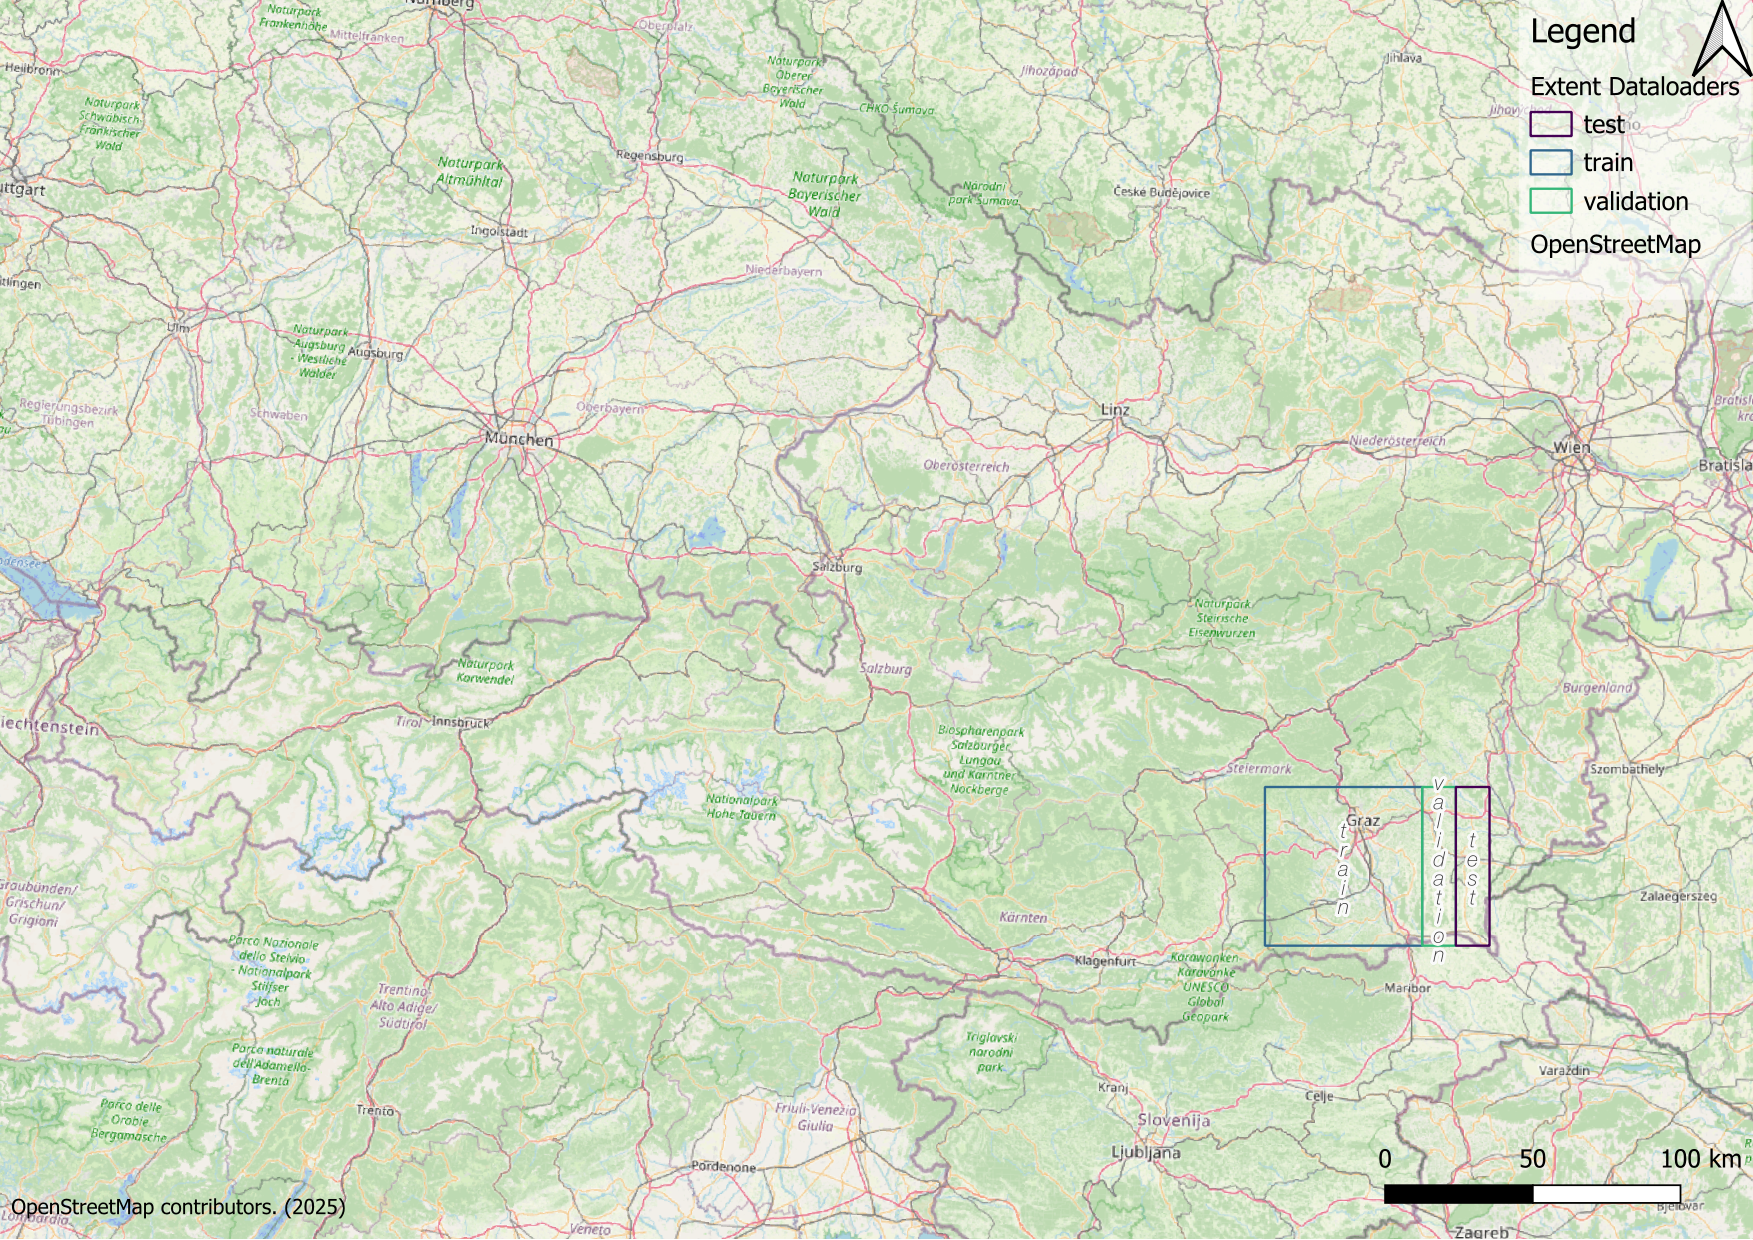
\includegraphics[width=1\linewidth]{Images_from_other_sources/uebersicht_at_low_dpi.jpg}
        \caption{Overview of the study area's location within Austria}
    \label{fig:overview_map}
\end{figure}

\begin{figure}
    \centering
    \includegraphics[width=1\linewidth]{Images_from_other_sources/detail_dataloader_orthophoto_low_res.jpg}
        \caption{Detailed overview of the study area}
    \label{fig:detail_overview_map}
\end{figure}

\par
The primary study area for this research is defined by the extent of the orthoimage tile with the ID 2024350 provided by the Bundesamt für Eich- und Vermessungswesen - BEV. It is located in Austria and covers an area of around 5040 square km around the City of Graz. Chosen for its diverse landscape that encompasses a mix of agricultural, rural, and urban land use types, it is home to several vineyards, orchards, forests, diverse sets of agricultural uses but also houses urban and mixed topographical settings. This heterogeneity provides a rich and challenging environment for testing the capabilities of semantic segmentation models on a fine-grained class schema. Figures \ref{fig:overview_map} and \ref{fig:detail_overview_map} provide an overview of the study area's location within Austria and the extent of the VHR and Data Loader extents for model training, validation and testing. \par
The selection of this exact extent was driven by the availability of high-quality VHR aerial ortho imagery provided by the  BEV, which serves as the primary remote sensing data source for the study. The approach can be used for the entire country of Austria, or the European Union, since the automated OSM data acquisition process is not the limiting factor. Using the proposed workflow restricts the analysis to the EU due to the INVEKOS Schläge Layer, which extends the information beyond the available OSM tag of landuse=farmland. \par
Hardware restrictions further limit the extent of the study area. One RGB-NIR orthophoto-tile uses around 42 gigabytes of disk space and holds 126 billion pixels. At 512 by 512 pixels, a single orthophoto-tile encompasses 480.651 unique tiles without overlap. Due to insufficient hardware, most of the model training is performed in a paid Google Colab with 15 GB of VRAM. Typically, one training epoch with 5.000 images and ground truth pairs takes around 1.5 hours to compute. Training on the entire dataset of one orthoimage tile would take 6 days, which exceeds the scope of this thesis, as the first research question requires this process to be repeated three consecutive times. Because of these limitations, a balance must be found between the tradeoffs of the model's access to diversity in training data and seen examples and computational restrictions. 
\subsection{Data Acquisition and Preprocessing}
\label{seq:data_acquisition}
A multi-source data strategy is adopted, integrating VHR aerial imagery with vector-based geospatial data from both crowdsourced and authoritative origins. To manage the high computational and memory requirements of processing large VHR images, the entire workflow is implemented using a tiling or sub-region approach. The overall Area of Interest (AOI) defined by the reference orthoimage is systematically divided into a grid of smaller, non-overlapping subregions, and all subsequent data acquisition and processing steps are performed independently on each subregion.
\subsubsection{Remote Sensing Imagery}
The primary remote sensing data consists of VHR orthoimagery for the specified study area, acquired from the BEV data portal. The imagery is provided in GeoTIFF format with four spectral bands separated into two files: Red, Green, Blue (RGB), and Near-Infrared (NIR) \parencite{BundesamtfurEich-undVermessungswesenOrthophotoFarbe2025}. Upon initial loading, key metadata, including the Coordinate Reference System (CRS), spatial resolution (GSD), and geographic extent (bounds), are extracted using the \textbf{rasterio} library in Python \parencite{GilliesRasteriogeospatialrasterPythonprogrammers2013}. This metadata establishes the foundational geometric reference for all subsequent data processing. \par
\subsubsection{OpenStreetMap Data}
OSM data serves as the primary source for a wide range of LULC features, particularly for built-up and natural environments. The data is acquired programmatically for each subregion's geographic extent using the \textbf{osmnx} Python library \parencite{BoeingModelingAnalyzingUrbanNetworksAmenitiesOSMnx2025}. The acquisition process is guided by the \texttt{osm\_class\_definitions} dictionary, which specifies a comprehensive set of key-value tag filters (e.g., \textit{{"building": "residential"}}, see Table \ref{tab:osm_definitions} for a detailed listing of key-value tags and respective geometry types for OSM data) to retrieve specific feature types  \parencite{OpenStreetMapcontributorsOpenStreetMap2025}.
A critical preprocessing pipeline is applied to the raw OSM vector data to prepare it for ground truth generation:
\begin{enumerate}
    \item \textbf{Reprojection:} The downloaded OSM data, which is by default in WGS84 (EPSG:4326), is reprojected to match the local CRS of the reference orthoimagery.
    \item \textbf{Geometric Buffering:} Since semantic segmentation requires polygonal masks, non-polygonal geometries from OSM must be converted. A buffering operation is applied to point and line features to create polygonal representations. The buffer distance is defined on a per-class basis (e.g., 5 meters for motorways, 1.5 meters for minor streams) to approximate the real-world footprint of these linear or point-based features \parencite{JordahlEtAlgeopandasgeopandasv0812020}.
    \item \textbf{Geometry Validation:} All geometries are processed using a \texttt{make\_valid} operation to correct any topological errors (e.g., self-intersections) that may exist in the raw data, ensuring their validity for subsequent overlay operations \parencite{JordahlEtAlgeopandasgeopandasv0812020}.
\end{enumerate}
\par

\subsubsection{INVEKOS Data}

To enhance the thematic detail and accuracy for agricultural classes, which are often coarsely represented in OSM, data from the Austrian \textbf{INVEKOS} system (Integrated Administration and Control System) is integrated. This authoritative dataset provides detailed, parcel-level information on agricultural land use \parencite{AgrarmarktAustriaINVEKOSSchlageOsterreich2024}.
\begin{enumerate}
    \item \textbf{Data Acquisition:} The INVEKOS data is loaded from a GeoPackage file containing parcel polygons, each with a specific thematic land use code (SNAR\_CODE).
    \item \textbf{Preprocessing:} The dataset is first clipped to the extent of each subregion to ensure spatial correspondence. The core preprocessing step involves a \textbf{thematic remapping}, where the numeric SNAR\_CODE of each parcel is translated into the unified, final class ID system of the thesis, as defined in the \texttt{snar\_code\_to\_final\_id\_map\_broad} dictionary. This step harmonizes the authoritative thematic labels with the broader class schema used for both OSM data and the final model training \parencite{JordahlEtAlgeopandasgeopandasv0812020}.
\end{enumerate}
\par
\subsection{Ground Truth Data Generation}
\label{seq:ground_truth_generation}
The final and most critical stage of the data preparation pipeline is the generation of a single, non-overlapping, and clean ground truth label mask for each subregion. This is achieved by fusing the preprocessed INVEKOS and OSM data through a novel vectorized hierarchical overlay process, designed to logically resolve conflicts between overlapping features from different sources and classes.
The process is governed by a strict, predefined \textbf{hierarchy} list, which dictates the priority of every LULC class. For instance, \texttt{building} features are given higher priority than \texttt{forest} features, meaning that a pixel cannot be labeled as both. The fusion operates as follows:
\begin{enumerate}
    \item \textbf{Data Combination:} For each subregion, the preprocessed INVEKOS and OSM GeoDataFrames are combined into a single dataset.
    \item \textbf{Iterative Hierarchical Overlay:} The combined dataset is processed in an iterative fashion, following the class priority defined in the hierarchy list.
    \begin{itemize}
        \item The highest-priority class is processed first. All its geometries are dissolved into a single (multi)polygon feature.
        \item  This dissolved geometry is then used as an "eraser." For the next class in the hierarchy, its geometries are first dissolved, and then the geometry of the higher-priority class is subtracted from it using a geometric \texttt{difference} operation available in the geopandas library \parencite{JordahlEtAlgeopandasgeopandasv0812020}.
        \item  The resulting, non-overlapping geometry for the current class is stored, and the "eraser" is updated by performing a \texttt{union} with the current class's original geometry.
        \item  This process repeats for every class down the hierarchy, ensuring that each subsequent class only occupies areas not already claimed by a higher-priority class.
    \end{itemize}
    \item \textbf{Vector-to-Raster Conversion:} The output of the hierarchical overlay is a single, clean GeoDataFrame of non-overlapping polygons. This vector dataset is then "burned" into a single-band raster file using the \texttt{rasterio.features.rasterize} function \parencite{GilliesRasteriogeospatialrasterPythonprogrammers2013}. 
\end{enumerate}

The resulting ground truth mask is a GeoTIFF where each pixel's integer value corresponds to its final \texttt{class\_id}, and which perfectly aligns with the original remote sensing imagery in terms of extent, resolution, and CRS. This final raster mask is the ground truth data used for training and evaluating the semantic segmentation models.






\subsubsection{OSM Data Processing}
The generation of ground truth from OpenStreetMap requires a systematic translation of its raw, tag-based vector data into analysis-ready polygons suitable for rasterization. As OSM features can be represented as points, lines, or polygons, a standardized preprocessing workflow is necessary to create a consistent geometric dataset. This workflow formalizes the rules for querying features from OSM and the geometric operations needed to convert them into meaningful polygonal footprints.

Table \ref{tab:osm_definitions} details the explicit processing rules for each of the 34 classes derived from OSM. For each class, the table specifies the tag filters used to query the data via the \texttt{osmnx} library. It also defines the accepted geometry types (e.g., `Polygon`, `LineString`). A key step in this process is the conversion of non-polygonal features into areas. For linear features like roads and railways, and point features like power towers, a buffering operation is applied to approximate their real-world extent. The buffer radius, as shown in the table, is class-dependent; for instance, a major highway (`Class ID 5`) receives a 5-meter buffer, whereas a minor unpaved track (`Class ID 7`) receives a 1.5-meter buffer. This ensures that the generated polygons are plausible representations of the features on the ground, a necessary step before they can be used in the hierarchical fusion process.

\begin{longtable}{@{}p{0.08\textwidth} p{0.2\textwidth} p{0.35\textwidth} p{0.15\textwidth} p{0.12\textwidth}@{}}
\caption{OSM Feature Class Definitions, Tags, and Geometric Processing Rules.}\\
\toprule
\textbf{Class ID} & \textbf{Class Name} & \textbf{OSM Tags (Key: [Values])} & \textbf{Geometry Types} & \textbf{Buffer (m) / Final ID} \\
\midrule
\endhead

\multicolumn{5}{l}{\textit{Urban / Built-up}} \\
\midrule
1 & Residential Building & `building': ['residential', 'house', 'apartments', 'semidetached\_house', 'terrace'] & Polygon, MultiPolygon & N/A \\
2 & Commercial/ Office Building & `building': ['commercial', 'office', 'retail'] & Polygon, MultiPolygon & N/A \\
3 & Industrial Building & `building': ['industrial', 'warehouse'] & Polygon, MultiPolygon & N/A \\
4 & Unspecified Building & `building': 'yes' & Polygon, MultiPolygon & N/A \\
\midrule
\multicolumn{5}{l}{\textit{Transportation}} \\
\midrule
5 & Paved Road (Motorway/Trunk) & `highway': ['motorway', 'trunk', 'primary'], `surface': ['asphalt', 'concrete', 'paved'] & LineString, MultiLineString & LineString: 5, MultiLineString: 5 \\
6 & Paved Road (Other) & `highway': ['secondary', 'tertiary', 'residential', 'service', 'unclassified', 'living\_street'], `surface': ['asphalt', 'concrete', 'paved'] & LineString, MultiLineString & LineString: 3, MultiLineString: 3 \\
7 & Unpaved Road & `highway': ['track', 'unclassified', 'residential', 'service', 'path'], `surface': ['dirt', 'gravel', 'unpaved', 'ground', 'sand'] & LineString, MultiLineString & LineString: 1.5, MultiLineString: 1.5 \\
8 & Parking Area (Area) & `amenity': 'parking' & Polygon, MultiPolygon & N/A \\
801 & Parking Area (Aisles) & `highway': 'service', `service': 'parking\_aisle' & LineString, MultiLineString & Final ID: 8, Buffer: 2.5 \\
9 & Railway (Area) & `landuse': 'railway' & Polygon, MultiPolygon & N/A \\
901 & Railway (Track) & `railway': ['rail', 'light\_rail', 'tram', 'subway'] & LineString, MultiLineString & Final ID: 9, Buffer: 3 \\
30 & Aerodrome & `aeroway': ['aerodrome', 'runway', 'taxiway', 'apron'] & Polygon, MultiPolygon, LineString, MultiLineString & LineString: 12.5 \\
\midrule
\multicolumn{5}{l}{\textit{Natural / Vegetation}} \\
\midrule
10 & Forest / Woodland & `natural': 'wood', `landuse': 'forest' & Polygon, MultiPolygon & N/A \\
11 & Grassland / Mown Grass & `natural': 'grassland', `landuse': ['grass', 'meadow'] & Polygon, MultiPolygon & N/A \\
12 & Heath / Scrub & `natural': ['heath', 'scrub'] & Polygon, MultiPolygon & N/A \\
13 & Bare Earth (Natural) & `natural': ['bare\_rock', 'mud', 'sand', 'shingle', 'scree'] & Polygon, MultiPolygon & N/A \\
14 & Wetland & `natural': 'wetland' & Polygon, MultiPolygon & N/A \\
15 & Cliff & `natural': 'cliff' & Polygon, MultiPolygon, LineString, MultiLineString & LineString: 2 \\
16 & Glacier & `natural': 'glacier' & Polygon, MultiPolygon & N/A \\
17 & Scree / Talus & `natural': 'scree' & Polygon, MultiPolygon & N/A \\
\midrule
\multicolumn{5}{l}{\textit{Water}} \\
\midrule
18 & River / Large Waterbody & `natural': 'water', `water': ['river', 'lake', 'reservoir', 'ocean'] & Polygon, MultiPolygon & N/A \\
19 & Stream / Canal / Drainage Ditch & `waterway': ['stream', 'canal', 'drain', 'ditch'] & LineString, MultiLineString & LineString: 1.5 \\
20 & Swimming Pool & `leisure': 'swimming\_pool', `amenity': 'swimming\_pool' & Polygon, MultiPolygon, Point, MultiPoint & Point: 3 \\
\midrule
\multicolumn{5}{l}{\textit{Agricultural}} \\
\midrule
21 & Agricultural Field (Generic) & `landuse': ['farmland', 'paddy'] & Polygon, MultiPolygon & N/A \\
22 & Orchard & `landuse': 'orchard' & Polygon, MultiPolygon & N/A \\
23 & Vineyard & `landuse': 'vineyard' & Polygon, MultiPolygon & N/A \\
24 & Allotments / Community Garden & `landuse': 'allotments' & Polygon, MultiPolygon & N/A \\
25 & Farmyard & `landuse': 'farmyard' & Polygon, MultiPolygon & N/A \\
26 & Greenhouse Horticulture & `landuse': 'greenhouse\_horticulture', `building': 'greenhouse' & Polygon, MultiPolygon & N/A \\
\midrule
\multicolumn{5}{l}{\textit{Infrastructure / Utilities}} \\
\midrule
27 & Power Transmission Tower & `power': 'tower' & Point, MultiPoint, Polygon, MultiPolygon & Point: 6 \\
28 & Windmill & `man\_made': 'wind\_turbine', `building': 'windmill' & Point, MultiPoint, Polygon, MultiPolygon & Point: 9 \\
29 & Substation & `power': 'substation' & Polygon, MultiPolygon & N/A \\
\midrule
\multicolumn{5}{l}{\textit{Other Developed Land}} \\
\midrule
31 & Quarry & `landuse': 'quarry' & Polygon, MultiPolygon & N/A \\
32 & Cemetery / Graveyard & `landuse': 'cemetery', `amenity': 'grave\_yard' & Polygon, MultiPolygon & N/A \\
33 & Recreational Ground/Park & `leisure': 'park', `landuse': 'recreation\_ground' & Polygon, MultiPolygon & N/A \\
34 & Sports Pitch/Court & `leisure': 'pitch' & Polygon, MultiPolygon & N/A \\
\bottomrule
\label{tab:osm_definitions} 
\end{longtable}


\subsubsection{Fusion with INVEKOS}
While OSM provides excellent spatial detail for many LULC classes, its thematic granularity for agricultural land use is often limited. To overcome this, the workflow integrates parcel data from the Austrian INVEKOS system, which provides authoritative, fine-grained thematic labels for agricultural parcels. The fusion of these two data sources is the cornerstone of the ground truth generation process, creating a hybrid dataset that leverages the strengths of both.

The first step in this fusion is to harmonize the INVEKOS thematic codes with the project's class schema. Table~\ref{tab:invekos_mapping} details this remapping process, specifying how each official INVEKOS `SNAR\_CODE` is mapped to a final, broader class ID presented in Table \ref{class_schema}. This creates two distinct but schema-aligned vector datasets: one from OSM and one from INVEKOS.

\begin{longtable}{@{}p{0.3\textwidth} p{0.1\textwidth} p{0.6\textwidth}@{}}
\caption{Mapping of INVEKOS SNAR Codes to Final Class IDs.}\\
\toprule
\textbf{Final Class Concept (OSM ID)} & \textbf{Final ID} & \textbf{Corresponding INVEKOS SNAR Codes} \\
\midrule
\endhead

Vineyards (OSM 23) & 23 & 901, 907, 906, 862 \\
\hline
Orchards / Fruit / Nurseries (OSM 22) & 22 & 817, 818, 813, 814, 820, 854, 832, 844, 831, 819, 828, 829, 830, 809, 855, 861, 860 \\
\hline
Forestry (OSM 10) & 10 & 863, 864, 964, 961 \\
\hline
Greenhouses (OSM 26) & 26 & 840, 837, 838, 839, 849, 850, 851, 852, 845, 846, 848, 847, 843 \\
\midrule
\multicolumn{3}{l}{\textit{INVEKOS Extensions (New Broad Class IDs)}} \\
\midrule
INV Arable AllFieldCrops & 35 & 138, 105, 109, 110, 142, 155, 111, 165, 145, 117, 118, 119, 113, 114, 112, 137, 181, 166, 157, 150, 149, 141, 146, 179, 120, 154, 758, 759, 651, 524, 519, 525, 527, 513, 528, 631, 769, 308, 214, 212, 213, 211, 210, 203, 626, 627, 209, 625, 624, 623, 628, 207, 751, 307, 301, 509, 510, 658, 310, 506, 538, 539, 680, 682, 689, 690, 536, 537, 540, 772, 752, 775, 657, 302, 303, 304, 535, 696, 768, 694, 697, 676, 106, 115, 638, 208, 206, 679, 634, 635, 633, 681, 135, 776, 184, 764, 116, 173, 107, 774, 661, 671, 686, 767, 125, 126, 129, 130, 131, 134, 139, 140, 143, 144, 148, 153, 156, 159, 160, 161, 164, 167, 168, 169, 170, 171, 174, 175, 176, 177, 178, 180, 182, 183, 185, 204, 205, 311, 520, 526, 529, 663, 664, 665, 763, 765, 182 \\
\hline
INV Grassland AllTypes & 36 & 717, 716, 715, 992, 636, 642, 701, 704, 707, 708, 710, 723, 637 \\
\hline
INV Fallow SetAside & 37 & 771, 721, 653, 959 \\
\hline
INV GLOEZ MixedAgriEnvFeatures & 38 & 360, 359, 366, 361, 364, 363 \\
\hline
INV SpecialtyCrop\_Hops & 39 & 821 \\
\hline
INV Other Or Unknown Detail & 0 & 810, 865, and any unmapped codes \\
\bottomrule
\label{tab:invekos_mapping} 
\end{longtable}


\subsubsection{Definition of the Fine-Grained Class Schema}
\label{sec:def_class_schema}
A foundational component of any semantic segmentation task is a clear and comprehensive class schema. Standard LULC schemas are often too coarse for the level of detail visible in VHR imagery. Therefore, a primary methodological step in this research was to develop a bespoke, fine-grained class schema capable of capturing the nuanced differences between land use and land cover types in the study area.

The resulting schema is a hybrid system comprising a total of 40 distinct categories. It was designed by integrating general-purpose urban and natural land cover classes, derived from the rich semantic tagging system of OpenStreetMap \parencite{BoeingModelingAnalyzingUrbanNetworksAmenitiesOSMnx2025}, with specialized, high-confidence agricultural land use classes sourced from the authoritative INVEKOS dataset \parencite{AgrarmarktAustriaINVEKOSSchlageOsterreich2024}. The full class schema, which forms the basis for all subsequent ground truth generation and model training, is detailed in Table~\ref{class_schema}. Each entry in the table specifies a unique final Class ID, a human-readable Class Name, the original data Source (OSM or INVEKOS), and a brief description. Crucially, a corresponding \texttt{hierarchy} list was manually defined, which dictates the priority of every class (e.g., 'building' \> 'forest') to logically resolve spatial conflicts during data fusion.\par

The core of the fusion is a vectorized hierarchical overlay process, implemented in the \texttt{merge\_and\_prioritize} function. This process systematically resolves spatial conflicts between the two datasets based on a manually defined class priority list, which gives INVEKOS agricultural data higher precedence over generic OSM agricultural tags. The process iterates through each class in order of its priority, dissolving its geometries and using a geometric `difference` operation to "cut away" any areas that have already been claimed by a higher-priority class. This ensures that every pixel in the final map is assigned one and only one class label, resulting in a clean, topologically correct, and logically consistent ground truth dataset ready for rasterization and model training. \par

The entire data acquisition, processing and exportation workflow, described in Sections \ref{seq:data_acquisition} and \ref{seq:ground_truth_generation} is depicted in Figure \ref{fig:data_processing_workflow}. 

\begin{longtable}
{c c c p{4cm}}
\caption{Class schema detailing the ID's, names, sources and description of the ground truth data}
\hline
\toprule
\textbf{Class ID} & \textbf{Class Name} & \textbf{Source} & \textbf{Description} \\
\endhead

\hline
0 & Unknown or Other INVEKOS Class & INVEKOS & Default ID for INVEKOS codes that do not map to a specific category, see Table \ref{tab:invekos_mapping}. \\
\hline
1 & Residential Building & OSM & building=residential, house, apartments, etc. \\
\hline
2 & Commercial/Office Building & OSM & building=commercial, office, retail. \\
\hline
3 & Industrial Building & OSM & building=industrial, warehouse. \\
\hline
4 & Unspecified Building & OSM & building=yes. \\
\hline
5 & Paved Road (Motorway/Trunk) & OSM & Major paved highways, buffered into polygons. \\
\hline
6 & Paved Road (Other) & OSM & Minor paved roads (secondary, residential, etc.), buffered. \\
\hline
7 & Unpaved Road & OSM & Dirt, gravel, or track roads, buffered. \\
\hline
8 & Parking Area & OSM & amenity=parking areas and buffered service=parking\_aisle lines. \\
\hline
9 & Railway & OSM & landuse=railway areas and buffered railway tracks. \\
\hline
10 & Forest/Woodland & OSM/INVEKOS & natural=wood or landuse=forest and see Table \ref{tab:invekos_mapping}. \\
\hline
11 & Grassland/Mown Grass & OSM & natural=grassland or landuse=grass. \\
\hline
12 & Heath/Scrub & OSM & natural=heath or scrub. \\
\hline
13 & Bare Earth & OSM & natural=bare\_rock, mud, sand, shingle. \\
\hline
14 & Wetland & OSM & natural=wetland. \\
\hline
15 & Cliff & OSM & natural=cliff. \\
\hline
16 & Glacier & OSM & natural=glacier. \\
\hline
17 & Scree/Talus & OSM & natural=scree. \\
\hline
18 & River/Large Waterbody & OSM & natural=water (rivers, lakes, etc.). \\
\hline
19 & Stream/Canal/Drainage Ditch & OSM & Buffered linear waterways (waterway=stream, canal, etc.). \\
\hline
20 & Swimming Pool & OSM & leisure=swimming\_pool. \\
\hline
21 & Agricultural Field (Crops) & OSM & Generic landuse=farmland. INVEKOS data is more specific. \\
\hline
22 & Orchard & OSM/INVEKOS & landuse=orchard and see Table \ref{tab:invekos_mapping}. \\
\hline
23 & Vineyard & OSM/INVEKOS & landuse=vineyard and see Table \ref{tab:invekos_mapping}. \\
\hline
24 & Allotments/Community Garden & OSM & landuse=allotments. \\
\hline
25 & Farmyard & OSM & landuse=farmyard. \\
\hline
26 & Greenhouse Horticulture & OSM/INVEKOS & landuse= greenhouse\_horticulture or building=greenhouse and see Table \ref{tab:invekos_mapping}. \\
\hline
27 & Power Transmission Tower & OSM & Buffered power=tower points. \\
\hline
28 & Windmill & OSM & Buffered man\_made=wind\_turbine points. \\
\hline
29 & Substation & OSM & power=substation areas. \\
\hline
30 & Aerodrome & OSM & aeroway areas and buffered lines (runways, taxiways). \\
\hline
31 & Quarry & OSM & landuse=quarry. \\
\hline
32 & Cemetery/Graveyard & OSM & landuse=cemetery. \\
\hline
33 & Recreational Ground/Park & OSM & leisure=park or landuse=recreation\_ground. \\
\hline
34 & Sports Pitch/Court & OSM & leisure=pitch. \\
\hline
35 & Broad Arable Land / Field Crops & INVEKOS & A broad category for all standard field crops (cereals, legumes, etc.), see Table \ref{tab:invekos_mapping} \\
\hline
36 & Broad Grassland & INVEKOS & A broad category for all types of permanent grassland and meadows, see Table \ref{tab:invekos_mapping}. \\
\hline
37 & Fallow Land / Set-aside & INVEKOS & A broad category for all types of fallow or set-aside agricultural land, see Table \ref{tab:invekos_mapping}. \\
\hline
38 & Mixed Agri-Environmental Features & INVEKOS & GLÖZ features like hedges, field copses, stone ridges, see Table \ref{tab:invekos_mapping}. \\
\hline
39 & Specialty Crop (Hops) & INVEKOS & A distinct category for hops, which have a unique visual signature, see Table \ref{tab:invekos_mapping}. \\
\hline
\label{class_schema}
\end{longtable}

\newpage
\begin{sidewaysfigure}
    \includegraphics[width=\textwidth]{own_images/Workflow.jpg}
    \caption{Data Processing \& Preparation Workflow}
    \label{fig:data_processing_workflow}
\end{sidewaysfigure}


\subsubsection{Data Splitting}
A robust evaluation of a model's ability to generalize to new, unseen areas requires a careful data splitting strategy that avoids data leakage from spatial autocorrelation. Therefore, instead of a simple random splitting of image patches, which can lead to overly optimistic performance estimates on geospatial data, this study employs a spatial splitting methodology \parencites[p.~1ff.]{FengEtAlInformationLeakageDeepLearningBasedHyperspectralImageClassificationSurvey2023}[]{StewartEtAlTorchGeoDeepLearningGeospatialData2024}.

As implemented in the \texttt{1\_dataloading\_RGBI} notebook, the entire geographic Area/Region of Interest (ROI) is partitioned into three distinct, non-overlapping \texttt{BoundingBox} regions for training, validation, and testing. A 70\%/15\%/15\% split of the ROI's total width is used to define the spatial extent of the training, validation, and test sets, respectively. This spatial separation ensures that the model is evaluated on geographic areas it has not seen during training, providing a more realistic assessment of its performance in a real-world deployment scenario and preventing any potential data leakage between the sets \parencite[p.~3.]{FengEtAlInformationLeakageDeepLearningBasedHyperspectralImageClassificationSurvey2023}. During the training phase, data loaders for each split are created using \texttt{torchgeo.samplers.RandomGeoSampler}. This library class is designed specifically for geospatial data and enables the random sampling of fixed-size patches (512x512 pixels) from within a given spatial ROI, ensuring that patches are sourced exclusively from the correct geographic partition \parencite{StewartEtAlTorchGeoDeepLearningGeospatialData2024}.
\subsection{Semantic Segmentation Models}
\subsubsection{Model Architectures}
To address the primary technical research question, this thesis will implement, train, and compare three state-of-the-art deep learning architectures. These models were selected to represent distinct and influential families of semantic segmentation networks identified in the literature review:
\begin{itemize}
    \item \textbf{U-Net:} A classic and highly effective symmetric encoder-decoder architecture, renowned for its ability to capture fine-grained details via skip connections that fuse low-level and high-level feature maps \parencite[p.~4]{YuanEtAlreviewdeeplearningmethodssemanticsegmentationremotesensingimagery2021}. Its design is particularly well-suited for precise localization in segmentation tasks \parencite[p.~2]{RonnebergerEtAlUNetConvolutionalNetworksBiomedicalImageSegmentation2015}.
    \item \textbf{DeepLabV3+:} A state-of-the-art model that utilizes atrous (dilated) convolutions within its Atrous Spatial Pyramid Pooling (ASPP) module. This allows it to probe an incoming feature map at multiple scales, effectively capturing multi-scale contextual information without losing spatial resolution, a critical capability for analyzing complex remote sensing scenes \parencites[p.~179]{LuoEtAlSemanticsegmentationagriculturalimagessurvey2024} [p.~8f.]{SertelEtAlLandUseLandCoverMappingUsingDeepLearningBasedSegmentationApproachesVHRWorldview3Images2022}.
    \item \textbf{SegFormer:} A modern, efficient, and powerful framework based on a hierarchical Vision Transformer (ViT) encoder and a lightweight multilayer perceptron (MLP) decoder. Its design avoids the fixed positional encodings common in other ViT-based models, which improves generalization across different testing resolutions, and its lightweight decoder is both fast and effective \parencite[p.~1]{XieEtAlSegFormerSimpleEfficientDesignSemanticSegmentationTransformers2021}.
\end{itemize}
All models are implemented using the open-source \texttt{segmentation-models-pytorch} library, which provides a flexible framework for instantiating these architectures with various backbones \parencite{IakubovskiiSegmentationModelsPytorch2019}. For all experiments, the model encoders are initialized with weights pre-trained on the ImageNet dataset, for the configurations see Table \ref{tab:model_architectures}. This transfer learning approach is standard practice and has been shown to accelerate model convergence and improve final performance, even when transferring from natural image domains to remote sensing tasks \parencite[p.~2f.]{PiresDeLimaMarfurtConvolutionalNeuralNetworkRemoteSensingSceneClassificationTransferLearningAnalysis2019}.
\begin{table}[H]
\centering
\caption{Model Architectures and configurations}
\label{tab:model_architectures}
\begin{tabular}{llll}
\toprule
Model Architecture & Encoder Name & Encoder Weights & Number Parameters \\
\midrule
Segformer & mit\_b3 & imagenet & 44M \\
Unet & efficientnet-b3 & imagenet & 10M \\
DeepLabV3Plus & efficientnet-b3 & imagenet & 10M \\
\bottomrule
\end{tabular}

\end{table}

\subsubsection{Training Procedure}
\label{sec:training_procedure}
The models are trained using a consistent procedure managed within a PyTorch framework, as detailed in the \texttt{1\_dataloading\_RGBI} notebook found in the complementary GitHub Repository (serving as an Interactive Appendix \url{https://github.com/Moritz-Langer/Master_Thesis/tree/main/Model_Training}).
\begin{itemize}
    \item \textbf{Hardware and Device:} Training is conducted in a Google Colab environment utilizing a CUDA-enabled Tensor Processing Unit (TPU V4) to accelerate the computationally intensive matrix operations involved in deep learning. The device is specified as \texttt{cuda} if available, otherwise defaulting to \texttt{cpu} for compatibility.
    \item \textbf{Optimizer:} The \textbf{AdamW} optimizer is used for all training procedures. It is an extension of the Adam optimizer that improves weight decay regularization by decoupling it from the gradient-based update, and it has become a standard and robust choice for training modern deep learning models \parencite[p.~7]{LoshchilovHutterDecoupledWeightDecayRegularization2017}. An initial learning rate of \texttt{1e-4} is used.
    \item \textbf{Loss Function:} A key challenge in this fine-grained classification task is the severe class imbalance present in the dataset. To address this, a \textit{composite loss function} is employed. This function is a weighted sum of \textbf{Focal Loss} and \textbf{Dice Loss}, both of which are designed to perform well in imbalanced scenarios \parencite[p.~8.]{SertelEtAlLandUseLandCoverMappingUsingDeepLearningBasedSegmentationApproachesVHRWorldview3Images2022}.
        \begin{itemize}
            \item \textbf{Focal Loss}, an evolution of cross-entropy, dynamically scales the loss by adding a modulating factor. This has the effect of down-weighting the loss contribution of easy, well-classified examples, thereby forcing the model to focus its training efforts on harder, often minority, class examples \parencite[chapter ~4.1.]{WangEtAlComprehensiveSurveyLossFunctionsMachineLearning2022}.
            \item \textbf{Dice Loss} is a region-based loss function that optimizes a very similar formula to the Intersection over Union (IoU) metric. It is particularly effective for segmentation tasks with imbalanced classes because its gradient is not dominated by the number of pixels in the majority class \parencite[Table 1, Formula 8]{Jadonsurveylossfunctionssemanticsegmentation2020}.
        \end{itemize}
    \end{itemize}

    This combined criterion provides a robust objective function that balances the need for pixel-wise accuracy with the structural similarity required for high-quality segmentation. An \texttt{ignore\_index} is used to ensure that background or no-data pixels do not contribute to the loss calculation during training. Each model is trained up to 35 epochs and after each epoch, the model is validated against the validation dataloader to prevent data leakage and biased mIoUs. The model checkpoint is exported if the mIoU exceeds that of previous epochs. Therefore, models with the best performing generalization capabilities are considered for further examination. 

\subsection{Experimental Design}
\label{sec:experimental_design}
To systematically address the research questions of this thesis, a series of controlled experiments are designed.

\subsubsection{Addressing Technical RQ 1 (Model Comparison)}

\label{sec:addressing_technical_rq1}
\paragraph{Question 1:} Which deep learning architecture (U-Net, DeepLabV3+, SegFormer) is most suitable for this task given the characteristics of the orthophoto data and the target class scheme?
\paragraph{Experimental Procedure:} To answer this question, a direct comparative analysis of the three selected model architectures will be conducted. Each model—U-Net, DeepLabV3+, and SegFormer—will be trained and evaluated under identical conditions to ensure a reproducible comparison. The models will be trained on the full 4-channel (RGB-NIR) imagery and the complete, fused OSM-INVEKOS ground truth dataset as prepared in Section \ref{seq:ground_truth_generation}. Performance will be rigorously benchmarked using the quantitative metrics outlined in Section \ref{sec:eval_metrics}, with a primary focus on the mean Intersection over Union (mIoU), class specific IoU and confusion matrices are provided, enabling class specific inspection of User's and Producer's Accuracy.
\paragraph{Hypothesis Testing:} This experiment directly tests the hypothesis that architectures designed for superior context aggregation, namely SegFormer and DeepLabV3+, will outperform the standard U-Net architecture. It is tested whether their mechanisms for capturing both global and multi-scale context \parencite[p.~8f.]{SertelEtAlLandUseLandCoverMappingUsingDeepLearningBasedSegmentationApproachesVHRWorldview3Images2022} will yield significantly higher IoU scores. The outcome of this experiment will determine the most suitable architecture to be used in subsequent experiments.

\subsubsection{Addressing Technical RQ 2 (NIR Band Impact)}
\label{sec:addressing_technical_rq2}
\paragraph{Question 2:} How does the integration of the infrared band contribute to the performance of the segmentation compared to using only RGB data?
\paragraph{Experimental Procedure:} This experiment is designed to assess the effect of the NIR Band on segmentation performance. The best-performing model architecture identified in the previous experiment (Section \ref{sec:addressing_technical_rq1}) will be selected. Two instances of this model will then be trained:
\begin{enumerate}
\item \textbf{Model A (RGB-NIR):} Trained on the full 4-channel (RGB and NIR) dataset.
\item \textbf{Model B (RGB-only):} Trained on a 3-channel dataset where the NIR band has been excluded.
\end{enumerate}
Both models will be trained with identical hyperparameters and pool of ground truth training data. A direct comparison of their performance metrics will be conducted, with a particular focus on the class-wise IoU scores for vegetation-related classes (e.g., Forest/Woodland, Grassland/Mown Grass, Agricultural Field) and classes that are spectrally confusable with vegetation. For further investigation confusion matrices will be provided.
\paragraph{Hypothesis Testing:} This experiment will test the hypothesis that the inclusion of the NIR band provides a significant performance uplift. As the NIR band is highly sensitive to chlorophyll and vegetation health \parencite[p.~180ff.]{LuoEtAlSemanticsegmentationagriculturalimagessurvey2024}, it is hypothesized that Model A will demonstrate significantly higher segmentation accuracy for all vegetation types and will be better able to separate vegetated surfaces from spectrally similar non-vegetated surfaces like bare earth or certain building materials.


\subsubsection{Addressing Technical RQ 3 (Challenging Classes Analysis)}
\label{sec:addressing_technical_rq3}
\paragraph{Question 3:} What types of challenges ( See Section \ref{sec:osm_limitations_challenges} and \ref{sec:challenges_fine_grained_LULC}: Class Complexity and Semantic Ambiguity, Intra-class Variability and Inter-class Similarity, Class Imbalance Issues, Spatial Context and Scale, Positional Inaccuracy, Incompleteness and Thematic Errors, Temporal Mismatches, Geometric and Semantic Ambiguity) do specific fine-grained classes from the class schema (Table \ref{class_schema} present in segmentation, and which classes are most affected?
\paragraph{Experimental Procedure:} This inquiry moves beyond quantitative scores to a qualitative analysis of model behavior. The experiment will use the quantitative results from the model comparison in Section \ref{sec:addressing_technical_rq1} as a starting point. Specifically, the confusion matrix and per-class IoU scores will be used to identify a subset of the most challenging classes (i.e., those with the lowest performance). For this subset, a detailed qualitative assessment will be performed. This involves the side-by-side visual inspection of randomized occurrences. The original orthophoto, the ground truth mask, and the model's prediction mask are used to diagnose the nature of the errors, such as detailed in Section \ref{sec:challenges_fine_grained_LULC} and \ref{sec:osm_limitations_challenges} \parencites [p.~13f.]{SertelEtAlLandUseLandCoverMappingUsingDeepLearningBasedSegmentationApproachesVHRWorldview3Images2022} [p.~339]{CostaEtAlSupervisedmethodsimagesegmentationaccuracyassessmentlandcovermapping2018}.
\paragraph{Hypothesis Testing:} This qualitative analysis directly investigates the hypothesis that performance will be lowest for classes that are semantically similar, defined by land use rather than land cover, are compositionally heterogeneous, or represent fine linear features. The visual evidence will be used to categorize the errors and determine which of these known challenges in remote sensing segmentation is the primary cause for the model's failure mode for each specific class.

\subsubsection{Addressing Application/Utility RQ (Landscape Characterization)}
\label{sec:addressing_app_rq}
\paragraph{Question 1:} Which fine-grained classes can be mapped with sufficient reliability for landscape characterization and which metrics are most appropriate for this assessment?
\paragraph{Experimental Procedure:} This experiment focuses on the practical interpretation and utility of the segmentation results. The class-wise IoU scores from the primary model will be analyzed to identify which of the fine-grained classes can be mapped with high confidence. A reliability threshold (e.g., IoU > 0.7) will be established to categorize classes as "reliably mapped" for practical applications.
\paragraph{Hypothesis Testing:} This will test the hypotheses that (1) some classes can be more reliably mapped than others, and tries to disentangle which classes are more reliable in the model's outputs. This is linked to the previous research question \ref{sec:addressing_technical_rq3} that qualitatively examines the reasons for confusion and error presented in Section \ref{sec:challenges_fine_grained_LULC}. The present research question examines results from a quantitative perspective.

\subsubsection{Addressing Ground Truth RQ 1 (Sources and Challenges)}
\label{sec:addressing_gt_rq1}
\paragraph{Question 1:} What are the sources for creating or acquiring a ground truth dataset related to Austrian agricultural land use classes, and what are the challenges and opportunities?
\paragraph{Experimental Procedure:} This research question is addressed directly by the data engineering methodology developed for this thesis, as detailed in Sections \ref{seq:data_acquisition} and \ref{seq:ground_truth_generation}. The experiment consists of the successful implementation of the described data fusion pipeline. The process involves programmatically querying OSM data via \texttt{osmnx} \parencite{BoeingModelingAnalyzingUrbanNetworksAmenitiesOSMnx2025}, preprocessing the vector features with \texttt{geopandas} \parencite{JordahlEtAlgeopandasgeopandasv0812020}, remapping authoritative INVEKOS agricultural codes, and fusing the two sources using a priority-based hierarchical overlay.
\paragraph{Hypothesis Testing:} The successful generation of a clean, detailed, multi-source ground truth GeoPackage file serves as the validation for the hypothesis. It confirms that the thematic granularity of OSM for agriculture is insufficient alone and that its spatial accuracy can be successfully enhanced by leveraging the parcel-level thematic information from INVEKOS, demonstrating that fusing the datasets is a viable and necessary strategy to create a high-quality ground truth dataset.
\subsubsection{Addressing Ground Truth RQ 2 (Class Granularity Impact)}
\label{sec:addressing_gt_rq2}
\paragraph{Question 2:} How does the granularity of classes within the ground truth data influence the achievable accuracy of the segmentation results?
\paragraph{Experimental Procedure:} This experiment is designed to test two related hypotheses concerning the impact of class granularity.
\begin{enumerate}
\item \textbf{To test Hypothesis 2.1:} Two separate models will be trained. \textbf{Model A} will be trained on the full, fine-grained class schema (40 classes). \textbf{Model B} will be trained on a thematically aggregated, coarser version of the ground truth (e.g., all building types merged into a single 'Building' class). The performance (mIoU, F1-Score) of each model will be evaluated on its respective test set.
\item \textbf{To test Hypothesis 2.2:} The predictions from the fully trained Model A will be thematically aggregated to match the coarse schema of Model B. The performance of these aggregated predictions will then be directly compared to the predictions from Model B on the same coarse test set.
\end{enumerate}
\paragraph{Hypothesis Testing:} The first experiment is expected to confirm Hypothesis 2.1: that Model A, when evaluated at its fine-grained level, will achieve a lower overall mIoU than Model B evaluated at its coarse level, simply due to the increased difficulty of the task. The second, more crucial experiment tests Hypothesis 2.2. This hypothesis posits that Model A, by being forced to learn more subtle and discriminative features to separate fine-grained classes, will ultimately yield more accurate classifications at the coarse level when its outputs are aggregated, compared to the model trained directly on the less informative, coarse labels.
\paragraph{ }
\subsection{Evaluation}
To rigorously assess the performance of the semantic segmentation models and systematically address the research questions posed in this thesis, a multi-faceted evaluation strategy is employed. This strategy combines objective quantitative metrics with structured qualitative analysis. As surveyed in Section \ref{sec:eval_metrics}, no single metric can holistically capture model performance, especially given the fine-grained nature of the 40-class schema (Table \ref{class_schema}  and the inherent challenges of the fused OSM-INVEKOS ground truth data. This section, therefore, outlines the specific metrics chosen for this study, justifies their selection in the context of the research objectives, and details the protocol for their application.

\subsubsection{Quantitative Metrics}
The quantitative evaluation will be based on a pixel-level comparison between the model predictions and the ground truth masks generated in Section \ref{seq:ground_truth_generation}. Building upon the metrics surveyed in Section \ref{sec:eval_metrics}, the following will be the primary measures of performance:
\begin{itemize} 
    \item\textbf{Mean Intersection over Union (mIoU):} This will serve as the primary top-level metric for comparing the overall performance of different model architectures (addressing Technical RQ 1) and the impact of the NIR band (Technical RQ 2). Its robustness to class imbalance and its status as the de-facto standard in semantic segmentation literature make it the most suitable metric for overall comparison \parencite [p.~31.]{LeiEtAlDeeplearningimplementationimagesegmentationagriculturalapplicationscomprehensivereview2024}.
    \item\textbf{Per-Class IoU and F1-Score:}For the best performing model architecture the F1-Score and Per-Class IoU allow for further investigation. Given the severe class imbalance in the dataset, overall metrics like mIoU can obscure poor performance on rare but potentially significant classes (e.g.,\textit{Windmill}, \textit{Substation}). Therefore, per-class IoU and F1-Scores will be computed and reported for all 40 classes. This is crucial for identifying challenging classes (Technical RQ 3) and assessing the model's utility for detailed landscape characterization (Application/Utility RQ). The F1-score, as the harmonic mean of precision and recall, is particularly valuable here for providing a balanced measure of performance on minority classes \parencite [p.~9.]{SertelEtAlLandUseLandCoverMappingUsingDeepLearningBasedSegmentationApproachesVHRWorldview3Images2022}.
    \item\textbf{Confusion Matrices:}A row-normalized and a confusion matrix with absolute values will be generated for the best-performing model and its comparisson to the RGB trained model. The purpose of this is not merely to report precision and recall, but to serve as a diagnostic tool. It will be the primary instrument for identifying specific patterns of misclassification (e.g., confusion between \textit{Paved Road (Other)} and \textit{Parking Area}, or between different vegetation types). This directly supports the qualitative analysis aimed at understanding \textit{why} certain errors occur \parencite [p.~8f.]{SertelEtAlLandUseLandCoverMappingUsingDeepLearningBasedSegmentationApproachesVHRWorldview3Images2022}.
\end{itemize}


\subsubsection{Qualitative Assessment}
To complement the quantitative scores and provide a deeper understanding of the models' failure modes, a structured qualitative assessment will be conducted. This is vital because quantitative metrics can sometimes be misleading; for instance, a model might achieve a reasonable IoU on a class like \textit{Forest/Woodland} while producing blurry and unnatural boundaries \parencite [p.~10.]{KaiserEtAlLearningAerialImageSegmentationOnlineMaps2017}. The qualitative protocol is designed to diagnose these nuanced issues and directly address the research questions concerning the nature of segmentation errors.
The protocol will proceed as follows:
\begin{itemize}
    \item\textbf{Selection of Case Studies:} Based on the per-class IoU scores 5 worst-performing classes will be selected for detailed visual inspection. This targeted approach ensures the analysis is focused on its most significant failures.
    \item\textbf{Error Analysis through Visual Comparison:} For each selected class, several representative samples of correct and incorrect predictions will be extracted from the test set. A three-panel layout will be used—showing the (1) RGB orthophoto, (2) ground truth mask, and (3) prediction mask—to facilitate a direct visual diagnosis of the error type, as detailed in Section \ref{sec:qual_assessment}.
    \item \textbf{Systematic Error Characterization:} The goal of this visual inspection is to systematically characterize the primary reason for failure for the challenging classes, linking the errors back to the challenges identified in the literature review (Section \ref{sec:challenges_fine_grained_LULC}). Specifically, the analysis will seek to determine if errors are primarily due to:
    \begin{itemize}
        \item True spectral/textural similarity (e.g., \textit{Unpaved Road} vs. \textit{Bare Earth}).
        \item Semantic ambiguity/contextual failure (e.g., misclassifying a \textit{Farmyard} that is visually similar to a \textit{Residential Building} with a large garden).
         \item  Geometric inaccuracies (e.g., poor boundary delineation for linear features).
        \item Potential errors in the OSM-derived ground truth labels.
    \end{itemize}    
\end{itemize}
This combination of quantitative and qualitative evaluation provides a comprehensive framework to not only judge the final performance but also to generate actionable insights into the strengths and weaknesses of state-of-the-art models when applied to a complex, fine-grained LULC classification task.

\clearpage % <--- Force a new page here
\section{Results}
\label{sec:results}
This chapter presents the empirical findings from the experiments detailed in Section 3.5. The results are systematically organized to first assess the characteristics of the generated ground truth dataset. Next, the performance of the selected deep learning architectures is compared, followed by a quantification of the specific impact of the Near-Infrared (NIR) band within the best-performing architecture. Following the quantitative evaluation, a qualitative assessment of the model output is performed. Lastly, a quantitative analysis is conducted to examine the effects of granularity on model performance, particularly when comparing models with different training regimes regarding class depth on their capabilities to distinguish coarse class schemes.
\subsection{Ground Truth Data Assessment}

A prerequisite for interpreting model performance is a thorough understanding of the training and evaluation data. The class area distributions for the training, validation, and test splits are visualized in Figures  \ref{fig:train_data_distribution_abs}, \ref{fig:train_data_distribution_log}, \ref{fig:test_data_distribution_log}, and \ref{fig:val_data_distribution_log}.
A critical characteristic revealed by these figures is the severe \textbf{class imbalance} inherent in the dataset. As shown in Figure \ref{fig:train_data_distribution_abs}, the dataset exhibits a classic "long-tail" distribution. A few classes dominate the landscape in terms of area; specifically, \textit{Forest/Woodland} covers over 900 km² in the training split, followed by the main agricultural classes (\textit{Broad Arable Land / Field Crops} and \textit{Broad Grassland}), each covering hundreds of square kilometers. Conversely, a large number of classes are extremely rare, with functionally important categories like \textit{Substation}, \textit{Power Transmission Tower}, and \textit{Specialty Crop (Hops)} each covering less than 0.1 km². Two classes are not present in the study area: \textit{glaciers} and \textit{windmills}. \par
This extreme imbalance, spanning over several orders of magnitude, has significant implications for model training and evaluation. As established in the literature, models trained on such datasets can become biased towards predicting the majority classes, as this strategy minimizes overall error \parencite [p.~4f.]{QinLiuReviewLandcoverClassificationVeryHighResolutionRemotelySensedOpticalImagesAnalysisUnitModelScalabilityTransferability2022}. This reality underscores the importance of using evaluation metrics that are robust to class imbalance, such as the mean Intersection over Union (mIoU) and per-class F1-scores, rather than relying solely on overall accuracy. The use of specialized loss functions, as described in Section 3.4.2, is also strongly justified by this data assessment. The consistent distribution across the training (Figures \ref{fig:train_data_distribution_abs}, \ref{fig:train_data_distribution_log}), testing (Figure \ref{fig:test_data_distribution_log}), and validation (Figure \ref{fig:val_data_distribution_log}) splits confirms that the spatial splitting methodology has produced representative subsets for model development and evaluation. \par
A qualitative assessment of the ground truth data characteristics will be conducted in Section \ref{sec:discussion_challenges_data}, since qualitative examples of the training data are detailed in the latter part of this thesis. A complementary GitHub Repository with further examples for exploration is found via this URL:
\url{https://github.com/Moritz-Langer/Master_Thesis}. Within the directory \textit{Inference\_Examples} there are three sets of five randomly selected examples displaying the orthophoto, ground truth data, model prediction and the difference map of ground truth to prediction, as well as respective class Producer's Accuracy and top three classes of confusion.
\begin{figure} [H]
    \centering
    \includegraphics[width=0.65\linewidth]{own_images/area_distribution_abs_train.png}
    \caption{Area Distribution per Class for the Train Datasplit}
    \label{fig:train_data_distribution_abs}
\end{figure}

\begin{figure} [H]
    \centering
    \includegraphics[width=0.65\linewidth]{own_images/area_distribution_train.png}
    \caption{Area Distribution per Class for the Train Datasplit logarithmically scaled}
    \label{fig:train_data_distribution_log}
\end{figure}

\begin{figure}[H]
    \centering
    \includegraphics[width=0.65\linewidth]{own_images/area_distribution_test.png}
    \caption{Area Distribution per Class for the Test Datasplit logarithmically scaled}
    \label{fig:test_data_distribution_log}
\end{figure}

\begin{figure}[H]
    \centering
    \includegraphics[width=0.65\linewidth]{own_images/area_distribution_validation.png}
    \caption{Area Distribution per Class for the Validation Datasplit logarithmically scaled}
    \label{fig:val_data_distribution_log}
\end{figure}




\subsection{Performance of Different Architectures}
To address the technical research question regarding the most suitable architecture for this fine-grained segmentation task, the U-Net, DeepLabV3+, and SegFormer models were trained and evaluated on the full RGB-NIR dataset. The overall performance metrics are summarized in Table \ref{tab:performance_model_architectures}. Exemplary training scripts can be found via the GitHub Repository. The training strategy was limited to a maximum of 35 epochs and 5.000 image examples randomly sampled per epoch and tested against the test data split. If the model's mIoU on the test dataset increased with the current epoch, the model checkpoint was saved at the end of the test. The number of epochs and volume of images was adopted due to hardware and time constraints and will be discussed further in Section \ref{sec:study_limitations}. \par
\begin{table}[H]
\centering
\caption{Performance comparison for Model Architectures}
\label{tab:performance_model_architectures}
\begin{tabular}{llrr}
\toprule
Model Architecture & Encoder Backbone & mIoU & Overall Accuracy \\
\midrule
UNet & efficientnet-b3 & 0.119 & 0.182 \\
DeepLabV3+ & efficientnet-b3 & 0.176 & 0.304 \\
SegFormer & mit\_b3 & \textbf{0.239} & \textbf{0.340} \\
\bottomrule
\end{tabular}
\end{table}
The results clearly indicate that the \textbf{SegFormer} architecture provides superior performance, achieving the highest mIoU of 0.239 and the highest Overall Accuracy of 0.340. This outcome strongly supports the hypothesis that architectures designed for advanced context aggregation are better suited for complex, fine-grained LULC classification. The Transformer-based encoder in SegFormer, with its ability to model global and long-range dependencies via the self-attention mechanism, proves more effective than the atrous convolutions of DeepLabV3+ and the standard convolutional structure of U-Net (Xie et al., 2021). The U-Net model, while renowned for precise localization, appears to struggle significantly with the semantic complexity of the 40-class schema, yielding the lowest mIoU. \par
A deeper, class-specific analysis (Table \ref{tab:class_specific_iou_models_bold}) reinforces this finding. SegFormer outperforms the other models in a majority of the classes, particularly on challenging categories that require contextual reasoning, such as \textit{Quarry}, \textit{Cemetery/Graveyard}, and \textit{Recreational Ground/Park}. \par
The confusion matrices (Figures \ref{fig:con_mat_unet}, \ref{fig:con_mat_segformer}, \ref{fig:con_mat_deeplab}) provide further insight. The matrix for SegFormer (Figure \ref{fig:con_mat_segformer}) shows a noticeably "cleaner" diagonal compared to the others, indicating higher recall across many classes. For instance, U-Net (Figure \ref{fig:con_mat_unet}) almost completely fails to identify many classes, broadly confusing them with majority categories like \textit{Forest/Woodland} or \textit{Broad Arable Land / Field Crops}. While DeepLabV3+ (Figure \ref{fig:con_mat_deeplab}) performs better, it still exhibits more widespread confusion than SegFormer. Based on this comprehensive assessment, SegFormer is definitively the most suitable architecture and will be used for all subsequent analyses.

\begin{table}[H]
\centering
\caption{Class-specific Intersection over Union for Different Models}
\label{tab:class_specific_iou_models_bold}
\begin{tabular}{lrrr}
\toprule
Class Name & UNet & DeepLabV3+ & SegFormer \\
\midrule
Aerodrome & 0.00000 & \textbf{0.01033} & 0.00593 \\
Agricultural Field (Crops) & 0.00001 & 0.00138 & \textbf{0.00633} \\
Allotments/Community Garden & 0.00000 & 0.00000 & 0.00000 \\
Bare Earth & 0.00000 & 0.00000 & 0.00000 \\
Broad Arable Land / Field Crops & 0.77282 & 0.77396 & \textbf{0.80200} \\
Broad Grassland & 0.35899 & \textbf{0.40551} & 0.39385 \\
Cemetery/Graveyard & 0.00000 & 0.44621 & \textbf{0.67330} \\
Cliff & 0.00000 & 0.00000 & 0.00000 \\
Commercial/Office Building & 0.00000 & \textbf{0.00402} & 0.00002 \\
Fallow Land / Set-aside & 0.00000 & \textbf{0.10932} & 0.06917 \\
Farmyard & 0.00944 & 0.00854 & \textbf{0.02472} \\
Forest/Woodland & 0.90402 & 0.90268 & \textbf{0.92534} \\
Glacier & 0.00000 & 0.00000 & 0.00000 \\
Grassland/Mown Grass & 0.02033 & \textbf{0.15415} & 0.15387 \\
Greenhouse Horticulture & 0.00000 & 0.13668 & \textbf{0.56555} \\
Heath/Scrub & 0.00000 & \textbf{0.00359} & 0.00159 \\
Industrial Building & 0.00000 & \textbf{0.02536} & 0.00057 \\
Mixed Agri-Environmental Features & 0.00000 & 0.00011 & \textbf{0.03065} \\
Orchard & 0.53378 & 0.44227 & \textbf{0.66970} \\
Parking Area & 0.00000 & 0.24081 & \textbf{0.29857} \\
Paved Road (Motorway/Trunk) & 0.00022 & 0.00000 & \textbf{0.01588} \\
Paved Road (Other) & 0.22975 & 0.25918 & \textbf{0.28608} \\
Power Transmission Tower & 0.00000 & 0.00000 & \textbf{0.03074} \\
Quarry & 0.00000 & 0.14966 & \textbf{0.44467} \\
Railway & 0.12912 & 0.31699 & \textbf{0.51764} \\
Recreational Ground/Park & 0.00000 & 0.00000 & \textbf{0.08736} \\
Residential Building & 0.00000 & 0.00227 & \textbf{0.00747} \\
River/Large Waterbody & 0.50814 & 0.28256 & \textbf{0.67821} \\
Scree/Talus & 0.00000 & 0.00000 & 0.00000 \\
Specialty Crop (Hops) & 0.00000 & 0.00000 & 0.00000 \\
Sports Pitch/Court & 0.00000 & 0.28405 & \textbf{0.29224} \\
Stream/Canal/Drainage Ditch & 0.00000 & 0.01513 & \textbf{0.06557} \\
Substation & 0.00000 & 0.00000 & \textbf{0.00387} \\
Swimming Pool & 0.00000 & 0.25738 & \textbf{0.27823} \\
Unknown or Other INVEKOS Class & 0.00000 & 0.00000 & \textbf{0.00315} \\
Unpaved Road & 0.00000 & 0.10952 & \textbf{0.16421} \\
Unspecified Building & 0.38520 & 0.37329 & \textbf{0.39670} \\
Vineyard & 0.43706 & 0.63522 & \textbf{0.69397} \\
Wetland & 0.00000 & 0.00000 & 0.00000 \\
Windmill & 0.00000 & 0.00000 & 0.00000 \\
\bottomrule
\end{tabular}
\end{table}
\newpage
\begin{figure}[H]
    \vspace*{-4cm} % Adjust the value as needed to move the figure up
    \hspace*{-4cm} % Adjust the value as needed to move the figure to the left
    \includegraphics[width=1.7\textwidth]{own_images/low_res_confusion_matrix_UNet_efficienet_b3_20250622_155114.jpg}
    \caption{Confusion Matrix for the UNet architecture}
    \label{fig:con_mat_unet}
\end{figure}


\newpage
\begin{figure}[H]
    \vspace*{-4cm} % Adjust the value as needed to move the figure up
    \hspace*{-4cm} % Adjust the value as needed to move the figure to the left
    \includegraphics[width=2.03\textwidth]{own_images/confusion_matrix_SegFormer_mit_b3_20250626_204750.png}
    \caption{Confusion Matrix for the SegFormer architecture}
    \label{fig:con_mat_segformer}
\end{figure}



\newpage
\begin{figure}[H]
    \vspace*{-4cm} % Adjust the value as needed to move the figure up
    \hspace*{-4cm} % Adjust the value as needed to move the figure to the left
    \includegraphics[width=1.7\textwidth]{own_images/low_res_confusion_matrix_DeeplabV3_efficienet_b3_20250622_132643.jpg}
    \caption{Confusion Matrix for the DeepLabV3+ architecture}
    \label{fig:con_mat_deeplab}
\end{figure}

\subsection{Impact of the NIR Band}

To quantify the contribution of the NIR channel (Technical RQ 2), the best-performing architecture, SegFormer, was trained and evaluated on both a 3-channel (RGB) and a 4-channel (RGB-NIR) version of the dataset.
As shown in Table \ref{tab:model_performance_comparison}, the inclusion of the NIR band provides a positive impact on overall performance. The mIoU increases from 0.223 to 0.239, and the Overall Accuracy rises from 0.312 to 0.340.
The NIR band boosts the performance for several key classes. \par
Table \ref{tab:class_metrics_comparison_combined} shows the F1-score for \textit{Quarry} increases significantly, likely because the NIR band helps to distinguish bare soil and rock from surrounding vegetation and urban materials. Similarly, \textit{Recreational Ground/Park} sees an improvement, as the NIR data helps to separate managed grass and trees from unmanaged, spectrally similar \textit{Forest/Woodland} and \textit{Grassland}. The performance on \textit{Greenhouse Horticulture} also improves, as the NIR signal can help differentiate the artificial structures from surrounding fields. \par
Interestingly, a few classes show slightly better performance with the RGB-only model. For \textit{Industrial Building}, the IoU drops precipitously with the NIR band. A possible explanation is that certain roofing materials have a unique spectral signature in the visible spectrum that becomes ambiguous when the NIR channel is added, confusing them with vegetation or soil. Another explanation is that the model has seen more examples for the RGB training run by pure chance. For classes like \textit{Vineyard} and \textit{Railway}, the strong geometric patterns (rows of vines, parallel tracks) may be so dominant in the RGB channels that the additional NIR information introduces minor noise without adding significant value. \par
Overall, the results confirm the hypothesis that integrating NIR data is beneficial for fine-grained LULC segmentation. It acts as a discriminator for vegetation and natural surfaces, resolving ambiguities that are difficult to overcome with RGB data alone.

\begin{table}[H]
\centering
\caption{Overall Model Performance Comparison}
\label{tab:model_performance_comparison}
\begin{tabular}{lrr}
\toprule
Metric & RGB & RGB + NIR \\
\midrule
Mean IoU & 0.22300 & \textbf{0.23853}  \\
Overall Accuracy & 0.31202 & \textbf{0.34015}  \\
\bottomrule
\end{tabular}
\end{table}

\begin{table}[H]
 \begin{adjustwidth}{-2cm}{}
\centering
\caption{Class-specific Metric Comparison (IoU and F1-Score) for RGB and RGB-NIR Model}
\label{tab:class_metrics_comparison_combined}
\begin{tabular}{l S[table-format=1.6, detect-weight] S[table-format=1.6, detect-weight] | S[table-format=1.6, detect-weight] S[table-format=1.6, detect-weight]}
\toprule
Class Name & {RGB IoU} & {RGB + NIR IoU} & {RGB F1-Score} & {RGB + NIR F1-Score} \\
\midrule
Aerodrome & 0.000000 & \textbf{0.005930} & 0.000000 & \textbf{0.011784} \\
Agricultural Field (Crops) & \textbf{0.008660} & 0.006330 & \textbf{0.017179} & 0.012588 \\
Allotments/Community Garden & 0.000000 & 0.000000 & 0.000000 & 0.000000 \\
Bare Earth & 0.000000 & 0.000000 & 0.000000 & 0.000000 \\
Broad Arable Land / Field Crops & 0.794780 & \textbf{0.802000} & 0.885658 & \textbf{0.890122} \\
Broad Grassland & 0.383900 & \textbf{0.393850} & 0.554809 & \textbf{0.565127} \\
Cemetery/Graveyard & 0.650610 & \textbf{0.673300} & 0.788329 & \textbf{0.804754} \\
Cliff & 0.000000 & 0.000000 & 0.000000 & 0.000000 \\
Commercial/Office Building & 0.000000 & \textbf{0.000020} & 0.000004 & \textbf{0.000048} \\
Fallow Land / Set-aside & 0.047640 & \textbf{0.069170} & 0.090951 & \textbf{0.129384} \\
Farmyard & \textbf{0.027300} & 0.024720 & \textbf{0.053155} & 0.048255 \\
Forest/Woodland & 0.920270 & \textbf{0.925340} & 0.958481 & \textbf{0.961225} \\
Glacier & 0.000000 & 0.000000 & 0.000000 & 0.000000 \\
Grassland/Mown Grass & 0.134380 & \textbf{0.153870} & 0.236926 & \textbf{0.266704} \\
Greenhouse Horticulture & 0.425980 & \textbf{0.565550} & 0.597457 & \textbf{0.722491} \\
Heath/Scrub & \textbf{0.002180} & 0.001590 & \textbf{0.004350} & 0.003184 \\
Industrial Building & \textbf{0.184020} & 0.000570 & \textbf{0.310842} & 0.001147 \\
Mixed Agri-Environmental Features & 0.003490 & \textbf{0.030650} & 0.006947 & \textbf{0.059479} \\
Orchard & \textbf{0.675530} & 0.669700 & \textbf{0.806347} & 0.802184 \\
Parking Area & 0.281550 & \textbf{0.298570} & 0.439393 & \textbf{0.459844} \\
Paved Road (Motorway/Trunk) & 0.008330 & \textbf{0.015880} & 0.016525 & \textbf{0.031258} \\
Paved Road (Other) & 0.275290 & \textbf{0.286080} & 0.431732 & \textbf{0.444889} \\
Power Transmission Tower & 0.000000 & \textbf{0.030740} & 0.000000 & \textbf{0.059656} \\
Quarry & 0.074590 & \textbf{0.444670} & 0.138830 & \textbf{0.615599} \\
Railway & \textbf{0.629170} & 0.517640 & \textbf{0.772382} & 0.682168 \\
Recreational Ground/Park & 0.002980 & \textbf{0.087360} & 0.005944 & \textbf{0.160683} \\
Residential Building & 0.006380 & \textbf{0.007470} & 0.012671 & \textbf{0.014831} \\
River/Large Waterbody & 0.591630 & \textbf{0.678210} & 0.743429 & \textbf{0.808254} \\
Scree/Talus & 0.000000 & 0.000000 & 0.000000 & 0.000000 \\
Specialty Crop (Hops) & 0.000000 & 0.000000 & {nan} & 0.000000 \\
Sports Pitch/Court & 0.269240 & \textbf{0.292240} & 0.424251 & \textbf{0.452294} \\
Stream/Canal/Drainage Ditch & 0.050430 & \textbf{0.065570} & 0.096021 & \textbf{0.123062} \\
Substation & 0.000000 & \textbf{0.003870} & 0.000000 & \textbf{0.007715} \\
Swimming Pool & 0.267810 & \textbf{0.278230} & 0.422471 & \textbf{0.435339} \\
Unknown or Other INVEKOS Class & \textbf{0.006840} & 0.003150 & \textbf{0.013578} & 0.006285 \\
Unpaved Road & \textbf{0.170010} & 0.164210 & \textbf{0.290610} & 0.282099 \\
Unspecified Building & 0.380220 & \textbf{0.396700} & 0.550951 & \textbf{0.568052} \\
Vineyard & \textbf{0.754940} & 0.693970 & \textbf{0.860358} & 0.819345 \\
Wetland & 0.000000 & 0.000000 & 0.000000 & 0.000000 \\
Windmill & 0.000000 & 0.000000 & 0.000000 & 0.000000 \\
\bottomrule
\end{tabular}
\end{adjustwidth}
\end{table}



\subsection{Analysis of Challenging Classes and Confusion Patterns}

\begin{table}[H]
\centering
\caption{Top five elements for class-specific Intersection over Union for the best performing architecture}
\label{tab:class_specific_iou_best}
\begin{tabular}{lr}
\toprule
Class Name & IoU Score \\
\midrule
Forest/Woodland & 0.925 \\
Broad Arable Land / Field Crops & 0.802 \\
Vineyard & 0.694 \\
River/Large Waterbody & 0.678 \\
Cemetery/Graveyard & 0.673 \\
\bottomrule
\end{tabular}
\end{table}


\begin{table}[H]
\centering
\caption{Bottom Five Elements for Class Specific Intersection over Union}
\label{tab:class_specific_iou_worst}
\begin{tabular}{lr}
\toprule
Class Name & IoU Score \\
\midrule
Commercial/Office Building & 0.00002 \\
Industrial Building & 0.00057 \\
Heath/Scrub & 0.00159 \\
Unknown or Other INVEKOS Class & 0.00315 \\
Substation & 0.00387 \\
\bottomrule
\end{tabular}
\end{table}


While the overall quantitative metrics provide a high-level summary of model performance, a deeper understanding of the system's strengths and weaknesses requires a qualitative investigation into the specifically challenging classes detailed in Table \ref{tab:class_specific_iou_worst}. This section complements the quantitative data by performing a diagnostic analysis of classes that exhibited low IoU scores or significant confusion in the previous experiments. By visually inspecting the model's predictions against the ground truth and the original orthophoto, we can identify the root causes of error, linking them back to the inherent challenges of fine-grained LULC segmentation, such as class complexity, data source anomalies, and the limitations of deep learning models.
The following subsections present a detailed analysis for five representative challenging classes, using the diagnostic plots generated from the best-performing model. Each plot includes the original RGB image, the ground truth mask, the model's prediction, and a difference map highlighting correctly classified pixels (green), false negatives (red) and NoData in Ground Truth masks (black). \par
A primary challenge observed was the model's difficulty in \textbf{distinguishing between the semantics of fine-grained subclasses} of buildings, particularly \textit{Commercial/Office Building} and \textit{Industrial Building}. \par
\textbf{Commercial/Office Building:} As shown in the diagnostic plot (Figure \ref{fig:qual_eval_commercial_building}) for this class, while the model correctly identifies most building footprints, it systematically confuses them with the \textit{Unspecified Building} class. The quantitative analysis reveals that of the pixels that should have been classified as 'Commercial/Office', 97.8\% of the misclassifications were assigned to \textit{Unspecified Building}. Visual inspection of the image examples in Figure \ref{fig:qual_eval_commercial_building} (e.g., Masks 1, 3, and 6) confirms this pattern. The model accurately delineates the building structures, although it shows some degree of under-segmentation, and fails to assign the more specific semantic label. This indicates a high degree of \textbf{inter-class similarity} and \textbf{intra-class variability} among building types; many commercial and residential buildings share similar roofing materials and architectural styles, making them spectrally indistinguishable. This issue is likely exacerbated by inconsistent tagging in the source OSM data, where similar-looking buildings might be tagged differently by various contributors and depending on different use-percentage thresholds. \par
\textbf{Industrial Building:} The issue is even more pronounced for the \textit{Industrial Building} class. The quantitative results show that a staggering 98.1\% of misclassified  \textit{Industrial Building}  pixels were incorrectly labeled as \textit{Unspecified Building}. The visual examples demonstrate that while the model correctly identifies the large, often flat-roofed structures characteristic of industrial sites (e.g., Masks 2, 5, and 6), it overwhelmingly defaults to the more general \textit{Unspecified Building }label. This is a classic symptom of \textbf{class imbalance}. The \textit{Unspecified Building} class is far more prevalent in the training dataset, causing the model to develop a strong bias towards it (Figure \ref{fig:train_data_distribution_abs}, \ref{fig:train_data_distribution_log}). The model recognizes the general characteristics of a \textit{building} but lacks a sufficient number of distinct examples of  \textit{Industrial}  structures to confidently classify them as a more specific—and rare—category. Similar to its performance with Commercial Buildings, the model tends to under-segment buildings, incorporating parts of surrounding structures (such as roads and grassland) into the geometry of the buildings. \par
The model's ability to accurately delineate buildings, as indicated by the patterns in the confusion matrices (Figure \ref{fig:con_mat_unet}, \ref{fig:con_mat_segformer}, \ref{fig:con_mat_deeplab}), suggests that the underlying issue stems from an imbalance in the data. This assertion is further supported by Figures \ref{fig:train_data_distribution_abs}, \ref{fig:train_data_distribution_log}, \ref{fig:test_data_distribution_log}, \ref{fig:val_data_distribution_log}, which illustrate the class distribution and highlight the imbalance among building-related class IDs. In the training dataset, the Unspecified Building class is situated near the 10² square kilometer mark on the x-axis, while the Residential Building class is close to the 10 square kilometer mark. In contrast, the Industrial and Commercial Building classes are positioned near the 1 square kilometer mark. This significant shift in orders of magnitude likely skews the model's performance, resulting in semantic errors in the fine-grained details of building classification.
\begin{figure}
    \centering
    \includegraphics[width=1.2\linewidth]{own_images/low_res_greater_100_sqm_diagnostic_2_Commercial_Office Building.jpg}
    \caption{Qualitative Evaluation of the Commercial/Office Building Class (Image, Ground Truth, Predictions, Difference Map)}
    \label{fig:qual_eval_commercial_building}
\end{figure}
\begin{figure}
    \centering
    \includegraphics[width=1.2\linewidth]{own_images/low_res_greater_100_sqm_diagnostic_3_Industrial Building.jpg}
    \caption{Qualitative Evaluation of the Industrial Building Class (Image, Ground Truth, Predictions, Difference Map}
    \label{fig:qual_eval_industrial_building}
\end{figure}

\par
The \textit{Heath/Scrub} class proved to be one of the most challenging natural vegetation categories, with an IoU of 0.00159. Unlike spectrally homogeneous classes, \textit{Heath/Scrub} is defined by its ecological composition—a heterogeneous mixture of low-lying bushes, grasses, and often sparse, taller trees.
The diagnostic plot Figure \ref{fig:qual_eval_heath_srub} reveals that the model's predictions reflect this underlying complexity. The confusion is distributed among \textit{Forest/Woodland} (55.6\%), \textit{Broad Grassland} (20.4\%), and \textit{Broad Arable Land} (9.2\%). Visual inspection of Masks 1 and 6 provides a clear diagnosis: the model is not necessarily "wrong" in a spectral sense; rather, it is classifying the constituent components of the \textit{Heath/Scrub} area. It correctly identifies the woody vegetation as \textit{Forest/Woodland} and the grassy patches as \textit{Broad Grassland}. The core issue is one of \textbf{class complexity} and semantic ambiguity. The ground truth label represents an abstract ecological concept, while the model operates on the literal land cover it observes pixel by pixel. The model struggles to learn the abstract spatial texture that defines "heathland" as distinct from its constituent parts, a fundamental challenge when moving from land cover mapping to land use. \par

\begin{figure}
    \centering
    \includegraphics[width=1.2\linewidth]{own_images/low_res_greater_100_sqm_diagnostic_12_Heath_Scrub.jpg}
    \caption{Qualitative Evaluation of the Heath/Scrub Class (Image, Ground Truth, Predictions, Difference Map}
    \label{fig:qual_eval_heath_srub}
\end{figure}

\begin{figure}
    \centering
    \includegraphics[width=1.2\linewidth]{own_images/low_res_greater_100_sqm_diagnostic_29_Substation.jpg}
    \caption{Qualitative Evaluation of the Substation Class (Image, Ground Truth, Predictions, Difference Map}
    \label{fig:qual_eval_substation}
\end{figure}


The \textit{Substation} class, representing a rare and functionally-defined type of infrastructure, had a correct classification rate near zero (0.4\%). The diagnostic plot illustrates a complete failure of the model to learn a coherent representation for this class. The confusion is spread across \textit{Grassland/Mown Grass} (29.8\%), \textit{Unspecified Building} (14.6\%), and \textit{Paved Road (other)} (13.3\%), indicating that the model has no consistent strategy for this class. \par

The visual examples (Figure \ref{fig:qual_eval_substation} reveal two primary causes for this failure:
\begin{enumerate}

    \item\textbf{Extreme Class Imbalance:} As a very rare feature in the landscape, \textit{Substation} suffers from a severe lack of training examples, preventing the model from learning its specific features.
    \item\textbf{Land Use vs. Land Cover Ambiguity}: A \textit{substation} is a land use, not a single land cover. As seen in Masks 3 and 6, a substation area is typically a composite of grass, gravel (impervious surface), and metallic technical infrastructure. The model correctly identifies these constituent land covers but fails to learn the specific spatial arrangement that defines the land use "substation." Furthermore, as seen in Masks 2 and 5, some substations are housed within buildings, leading to extreme \textbf{inter-class similarity} with the \textit{Unspecified Building} class.
\end{enumerate}
\par
By design, the \textit{Unknown/Other INVEKOS} class (ID 0) serves as a repository for agricultural parcels from the authoritative data that could not be mapped to any other defined category. As expected, the model's performance on this class was effectively zero, with confusion being spread across \textit{Broad Arable Land} (35.5\%),\textit{Vineyard} (32.3\%), and \textit{Broad Grassland} (19.6\%). 
This result is not a model failure but rather a validation of the data's complexity. The diagnostic plot (Figure \ref{fig:qual_eval_unknown_other_invekos}) for this class is illuminating. It showcases parcels that are visually ambiguous or appear to be data errors in the source labeling. Mask 2, for example, shows a large, uniform field that the model classifies as \textit{Broad Arable Land}, which appears visually correct, suggesting the original label may have been anomalous. Mask 3 shows a parcel that appears texturally very similar to an orchard or vineyard, which is reflected in the model's confusion with the \textit{Vineyard} class. This "catch-all" class therefore represents the long tail of real-world complexity, including labeling errors, transitional land uses, and spectrally ambiguous agricultural stages that do not fit neatly into a predefined schema. The model's inability to form a coherent representation for this class is a direct reflection of the inherent inconsistency of the training samples labeled with this ID. \par
Finally, a recurring artifact is visible across many of the prediction masks: straight, grid-like edges that do not correspond to features on the ground (e.g., \textit{Heath/Scrub} Mask 1, \textit{Substation} Mask 3). These are edge effects resulting from the 512x512 pixel tiling strategy used by the GridGeoSampler. While this does not appear to be the primary cause of semantic confusion, it is a notable model behavior related to the loss of broader spatial context at the boundaries of the training patches.

\begin{figure}[H]
    \centering
    \includegraphics[width=1.2\linewidth]{own_images/low_res_greater_100_sqm_diagnostic_0_Unknown_Other INVEKOS.jpg}
    \caption{Qualitative Evaluation of the Unknown/Other Invekos (Image, Ground Truth, Predictions, Difference Map}
    \label{fig:qual_eval_unknown_other_invekos}
\end{figure}





\subsection{Influence of Class Granularity on Performance}

\begin{table}[H]
\centering
\caption{Remapping from Existing Schema to Target Schema}
\label{tab:remapping_schema_simple}
\begin{tabular}{ c l p{5cm} }
\hline
\textbf{New Class ID} & \textbf{New Class Name} & \textbf{Original Class IDs Mapped to New ID} \\
\hline
0 & Unknown/Background & 0 \\
\hline
1 & Buildings & 1, 2, 3, 4, 26 \\
\hline
2 & Roads & 5, 6, 7 \\
\hline
3 & Trees & 10, 22 \\
\hline
4 & 'Artificial' ground other than road & 8, 9, 20, 25, 27, 28, 29, 30, 31, 32, 34 \\
\hline
5 & 'Natural' ground covered by vegetation & 11, 12, 14, 21, 23, 24, 33, 35, 36, 37, 38, 39 \\
\hline
6 & Water & 18, 19 \\
\hline
7 & Bare Ground & 13, 15, 16, 17 \\
\hline
\end{tabular}
\end{table}

A central hypothesis of this thesis is that training a semantic segmentation model on a highly detailed, fine-grained class schema, while inherently more challenging, can force the model to learn more discriminative and robust features. These learned features, in turn, may lead to superior performance even when the model's output is evaluated at a coarser, more traditional level of aggregation. To investigate this, a two-part experiment was conducted as outlined in the methodology. The first part compares the performance of a model trained on the fine-grained schema against one trained on a coarse schema. The second, more crucial part, compares the aggregated output of the fine-grained model against the direct output of the coarse model.
For this analysis, "Model A" refers to the best-performing SegFormer model trained on the full, 40-class fine-grained schema. "Model B" refers to an identical SegFormer architecture trained from scratch on the 8-class coarse schema defined in Table \ref{tab:remapping_schema_simple}.


% Table 2: Evaluation Summary for Coarse and Fine-to-Coarse Models (Latest Entries)
\begin{table}[H]
\centering
\caption{Evaluation Summary for Coarse, Fine-to-Fine and Fine-to-Coarse Models}
\label{tab:evaluation_fine_to_coarse}
\begin{tabular}{lrr}
\toprule
    Model Type &   mIoU &  Overall Accuracy \\
\midrule
        Coarse & 0.4606 &            0.5501 \\
        Fine-to-Fine & 0.2385 & 0.3401 \\
Fine-to-Coarse & \textbf{0.4842} &            \textbf{0.5696} \\
\bottomrule
\end{tabular}
\end{table}

The first step confirms the intuitive expectation that a classification task becomes more difficult as the number of classes increases. As shown in the evaluation summaries, Model A, when evaluated on its native 40-class fine-grained test set, achieved a mean Intersection over Union (mIoU) of 0.239. In contrast, Model B, evaluated on its native 8-class coarse test set, achieved a significantly higher mIoU of 0.461. The results summarized in Table \ref{tab:evaluation_fine_to_coarse} directly supports Hypothesis 2.1, confirming that the overall performance, as measured by standard metrics, is lower for the more complex fine-grained task. This is an expected outcome, as the potential for inter-class confusion and the impact of class imbalance are far greater when distinguishing between 40 categories compared to just eight.
The core of this investigation lies in comparing the aggregated predictions of the fine-grained model (Model A) against the direct predictions of the coarse-grained model (Model B). This allows for a direct test of Hypothesis 2.2 from Section \ref{sec:addressing_gt_rq2}. The results of this comparison are summarized in Table \ref{tab:evaluation_fine_to_coarse} and are visualized in the confusion matrices in Figure \ref{fig:con_mat_fine_coarse} (Model A, aggregated) and Figure \ref{fig:con_mat_coarse} (Model B, direct).
The aggregated fine-to-coarse model (Model A) achieved an mIoU of 0.484, whereas the model trained directly on the coarse schema (Model B) achieved an mIoU of 0.461. While both models demonstrate strong performance, the model trained on the Fine-to-Coarse strategy shows a slight advantage in the overall mIoU score. However, a deeper analysis of the per-class IoU scores and the confusion matrices reveals a more nuanced picture.
\begin{figure}
    \centering
    \includegraphics[width=0.7\linewidth]{own_images/coarse_confusion_matrix_SegFormer_mit_b3_20250629_092703.png}
    \caption{Confusion Matrix for the Coarse trained model}
    \label{fig:con_mat_coarse}
\end{figure}
\begin{figure}
    \centering
    \includegraphics[width=0.7\linewidth]{own_images/fine_to_coarse_confusion_matrix_SegFormer_mit_b3_20250628_203226.png}
    \caption{Confusion Matrix for the Fine-to-Coarse trained model}
    \label{fig:con_mat_fine_coarse}
\end{figure}
\par
\textbf{Analysis of Confusion Matrices:}
\begin{itemize}
    \item Model A (Fine-to-Coarse): The confusion matrix for the aggregated fine-grained model shows remarkably strong performance on the dominant natural land cover classes. The Trees class achieves a producer's accuracy of 95.0\%, and the 'Natural' ground covered by vegetation class achieves 95.7\%. The Buildings class is also robust at 92.8\%. The primary sources of confusion are concentrated in the more ambiguous or less common classes. For example, the 'Artificial' ground other than road class shows significant confusion, with its pixels being misclassified as Roads (4.3\%) and 'Natural' ground covered by vegetation (20.7\%). This suggests that the model, despite its fine-grained training, still struggles to separate spectrally similar man-made and natural ground covers. Similarly, the Bare Ground class is heavily confused with Trees (46.0\%), likely due to shadows or dark soil appearing spectrally similar to forested areas.
    \item Model B (Coarse): The model trained directly on the coarse schema exhibits similar overall patterns but with subtle, important differences. While its performance on Trees (95.4\%) and 'Natural' ground covered by vegetation (95.4\%) is comparable to Model A, it shows less confusion for some of the ambiguous classes. For instance, 'Artificial' ground other than road, Model B  has a lower producer's accuracy (35.3\% vs. Model A's aggregated 56.3\%). However, it achieves higher Producer's Accuracy in the Road class (56\% compared to 48\% for Model A).
\end{itemize}

\begin{table}[H]
\centering
\caption{Per-Class IoU for Fine-to-Coarse and Coarse Models}
\label{tab:per_class_iou_fine_coarse}
\begin{tabular}{lrr}
\toprule
                            Class Name &  IoU (Fine to Coarse) &  IoU (Coarse) \\
\midrule
                    Unknown/Background &                \textbf{0.0032} &        0.0000 \\
                             Buildings &                \textbf{0.7929} &        0.7798 \\
                                 Roads &                \textbf{0.3676} &        0.3586 \\
                                 Trees &                0.9091 &        \textbf{0.9114} \\
   'Artificial' ground other than road &                \textbf{0.3343} &        0.2154 \\
'Natural' ground covered by vegetation &                \textbf{0.9149} &        0.9132 \\
                                 Water &                \textbf{0.5513} &        0.5062 \\
                           Bare Ground &                0.0000 &        0.0000 \\
\bottomrule
\end{tabular}
\end{table}

\textbf{Interpretation of Results:}
The results provide support for Hypothesis 2.2. While the aggregated fine-grained model (Model A) did not unequivocally outperform the coarse-trained model (Model B) in terms of class-specific IoU, it demonstrated superior or comparable performance in most classes. For instance, Model A achieved a higher IoU for 'Artificial' ground other than road (0.334 vs. 0.215) and Water (0.551 vs. 0.506).
This suggests that forcing the model to learn the subtle distinctions between fine-grained subclasses—such as separating Orchards and Vineyards from Forests—provides it with a more robust set of features for the broader Trees category. Similarly, learning to separate various types of roads and parking areas gives it a better foundation for identifying 'Artificial' ground other than road.
In conclusion, the hypothesis that a fine-grained training approach leads to universally superior coarse-level performance was not fully confirmed by the Class Specific IoU metric as shown in Table \ref{tab:per_class_iou_fine_coarse}, the per-class analysis indicates that this strategy offers significant advantages for most classes and in the aggregated results of the mIoU (Table \ref{tab:evaluation_fine_to_coarse}). The fine-grained training appears to imbue the model with more discriminative power for certain ambiguous categories and it does translate to a slightly higher overall score in this specific experimental setup. 
\clearpage % <--- Force a new page here
\section{Discussion}
The preceding chapters have established a rigorous methodological framework and presented a detailed quantitative and qualitative analysis of the experimental results. This chapter moves from the objective reporting of \textit{what} was found to the critical interpretation of \textit{what these findings mean}. It serves as the culmination of the thesis, synthesizing the results to answer the initial research questions, contextualizing the findings within the existing body of academic literature, and critically reflecting on the entire research process.
This discussion is structured to first interpret the specific outcomes of each experiment, addressing the performance of the model architectures, the contribution of the NIR band, the profound challenges arising from the fine-grained class schema and the use of multi-source ground truth data, the implications of class granularity, and the ultimate utility of the generated maps. Following this interpretation, the chapter will outline the study's limitations and conclude by articulating the principal implications and contributions of this research to the fields of remote sensing and geoinformation science.
\subsection{Interpretation of Results}
\subsubsection{Model Architecture Performance}
\label{sec:discussion_model_architecture}
The comparative analysis of the U-Net, DeepLabV3+, and SegFormer architectures provided a clear answer to the first technical research question. The SegFormer model, a modern Transformer-based architecture, demonstrated superior performance across nearly all quantitative metrics, achieving the highest mean Intersection over Union (mIoU). This finding empirically supports the hypothesis that architectures designed for advanced context aggregation are better suited for highly complex, fine-grained segmentation tasks. The strength of the SegFormer architecture lies in its Transformer encoder, which utilizes a self-attention mechanism to model global dependencies within the image \parencite[p.~2, 4.]{XieEtAlSegFormerSimpleEfficientDesignSemanticSegmentationTransformers2021}. Unlike traditional CNNs, which build context through a hierarchy of local receptive fields, the Transformer can assess the relationship between distant pixels in a single step. This is a decisive advantage when classifying ambiguous features whose identity is determined by broader spatial context. For instance, distinguishing a \textit{Farmyard} from a \textit{Parking Area} may depend on identifying surrounding agricultural fields versus commercial buildings. The SegFormer's ability to capture this global context provides a more robust foundation for making such nuanced distinctions compared to the more localized context windows of CNN-based models. \par
It is crucial, however, to contextualize these results within the constraints of this study. The training was limited to a maximum of 35 epochs with 5000 images per epoch, a constraint imposed by the available computational hardware and project timeline. It is conceivable that with a significantly larger training budget (i.e., more epochs and a larger batch size, larger study area extent), the performance gap between the architectures might change. The applied combination of chosen loss functions might lead to a performance increase within the minority classes, due to low sampling probability under the current circumstances. This negligible chance of sampling for minority classes can significantly contribute to the occlusion of certain classes in the model's outputs. Either the model has not seen the classes and their characteristics at the long end of the distribution or the exposure was minimal, making it impossible to establish a robust representation of said classes.
\par 
Nevertheless, the superior efficiency and performance of SegFormer under these limited conditions are themselves a significant finding. It suggests that Transformer-based models may not only offer a higher performance ceiling but also a faster path to convergence, which is a critical practical consideration for researchers with finite computational resources. 
\par The contribution of this analysis is therefore twofold: it \textbf{provides empirical validation} for the \textbf{suitability} of \textbf{Transformer architectures} in a \textbf{novel, highly granular LULC context} in Austria, and it underscores their practical \textbf{advantages in computationally constrained research environments}.
\subsubsection{NIR Band Contribution}
The study designed to evaluate the impact of the Near-Infrared (NIR) band yielded an unequivocal result: the \textbf{inclusion of the NIR channel provided a statistically significant improvement} in segmentation performance. This was particularly evident in the increased accuracy for many vegetation-related classes, confirming the hypothesis that the NIR band provides critical, non-redundant spectral information for distinguishing between different types of plant life. This aligns perfectly with the common sense in remote sensing, where the NIR band's sensitivity vegetation is a cornerstone of vegetation analysis \parencite[p.~183]{LuoEtAlSemanticsegmentationagriculturalimagessurvey2024}. \par
Parallel to the limitations due to hardware and time constraints mentioned in Section \ref{sec:discussion_model_architecture} on the model training strategy, the findings have to be regarded with caution, since it is expected that models have not fully converged yet. All evaluations of the different models trained for this analysis potentially profit from increasing the scale of the training procedure, exposing the model to more diverse representations of class-specific features and phenotypes. \par
The finding of improved performance when including the NIR Band invites a discussion on the trade-off between performance gain and the added overhead of using multispectral data extending beyond RGB channels. The inclusion of a fourth band increases data storage requirements and computational load during training. While in this study a performance benefit was percieved, this may not justify the inclusion of the NIR band for all applications. For a use case focused classes with negligible differences in performance depicted in Table \ref{tab:class_metrics_comparison_combined}, the added value of the NIR band might be minimal, and an RGB-only approach could be more efficient. Conversely, for any application involving agriculture, forestry, ecology, or environmental monitoring, this analysis demonstrates that the inclusion of the NIR band is beneficial. The contribution of this analysis is to provide a quantitative basis for this use-case-specific decision.

\subsubsection{Challenges with Fine-Grained Classes and OSM Data}
\label{sec:discussion_challenges_data}
The detailed qualitative and quantitative analysis of the per-class results reveals complex interconnected challenges. The model's failures are rarely attributable to a single cause; rather, they arise from a confluence of issues rooted in the class schema, the quality of the source data, and the inherent limitations of the learning process itself, especially as previously mentioned, due to the abbreviated training strategy adopted in this thesis. The following discussion focuses on the applied data acquisition and processing workflow, its source data quality and restrictions, as well as the utilized class schema. Three sets of five examples per class can be found in the associated GitHub Repository (\url{https://github.com/Moritz-Langer/Master_Thesis/tree/main/Inference_Examples}).
\paragraph{Class Complexity, Semantic Ambiguity, and Functional Definitions} A primary source of error was the model's struggle with classes defined by human function (land use) rather than physical appearance (land cover). This was most evident for classes like \textit{Recreational Ground/Park}, \textit{Allotments/Community Garden}, and \textit{Farmyard}, which were systematically misclassified as their primary land cover components—\textit{Forest/Woodland} or \textit{Grassland}. This confirms the classic challenge that pixel-based classifiers cannot easily infer abstract human concepts like "recreation" \parencite[p.~313]{KotaridisLazaridouRemotesensingimagesegmentationadvancesmetaanalysis2021a}. This was also the case for the \textit{Aerodrome} class, which, being a rural airfield, was classified as \textit{Broad Grassland} due to the dominance of its physical cover over its functional context. The composition of land-use classes from different individual land-cover features adds explanatory power to the challenge of occlusion or rare prediction of certain minority classes, further highlighting the inter-connected nature of challenges present in high-granularity class schemas for semantic segmentation in the context of LULC classification.
\paragraph{Intra-class Variability and Inter-class Similarity} These two issues were deeply intertwined. High intra-class variability was a major problem for ecologically heterogeneous classes like \textit{Heath/Scrub} and \textit{Wetland}, which are defined by a composite mixture of grass, shrubs, trees, and water. The model tended to classify the constituent parts rather than the abstract whole. Simultaneously, high inter-class similarity plagued many classes, most notably the failure to robustly distinguish between \textit{Unpaved Road} and \textit{Paved Road (Other)}, as well as among the different building subclasses which often share similar roofing materials. This challenge is related to the semantic ambiguity and fuzziness of the semantic class-specific delineation of their representations.
\paragraph{Class Imbalance Issues} The impact of severe class imbalance was the most decisive factor leading to the complete failure of the model to learn rare object classes. This was starkly illustrated by the near-zero accuracy for \textit{Power Transmission Tower}, \textit{Substation}, \textit{Cliff}, and \textit{Bare Earth}. The training dataset, reflecting the real world, contains millions of pixels of forests and fields for every few hundred pixels of a power tower. Faced with this extreme imbalance and a limited total training volume due to hardware constraints, the model's optimization process naturally prioritizes the majority classes, effectively ignoring the rare ones to minimize the overall loss function \parencite[p.~7934]{BhatEtAlRobustlossfunctionclassimbalancedsemanticsegmentationimageclassification2023a}. This is countered by the combination of loss functions, which inherently weight minority classes higher than majority classes. However, the severe imbalance leads to low exposure of the model to the classes at the long-tailed end of the distribution and, therefore, to a non-representative representation of the features, making it impossible for the model to predict this class.
\par
Data quality-specific shortcomings of the training data stemming from the proposed data acquisition and processing workflow are detailed below:
\paragraph{Ground Truth Data Quality: The OSM Contribution} This study powerfully underscores that in real-world applications, the quality of the training data is often a more significant constraint than the sophistication of the model. The automated ground truth generation pipeline, while necessary for scalability, directly inherited and in some cases amplified issues from the source OSM data.
\begin{itemize}
\item \textbf{Inconsistent Tagging and Thematic Errors:} The failure to distinguish between building types is a clear example of inconsistent tagging within OSM. Similarly, the finding that \textit{Paved Road (Other)} was classified more accurately than the supposedly higher-priority \textit{Paved Road (Motorway/Trunk)} points directly to thematic errors in the source data. This is also present for the \textit{Building} specific classes.
\item \textbf{Positional Inaccuracy and Geometric Ambiguity:} The use of fixed-width buffering for linear features is a necessary but imperfect heuristic. This introduced geometric noise, creating training masks that did not perfectly align with the features in the imagery, contributing to blurry boundaries and confusion with adjacent classes.
\item \textbf{Temporal Mismatches:} The complete failure of the \textit{Bare Earth} class is a strong indicator of a temporal mismatch between the OSM data and the more recent orthoimagery.
\item \textbf{Semantic Redundancy from Data Fusion:} A critical, methodological finding was the negative impact of semantic redundancy. The model’s failure to learn the OSM-derived \textit{Agricultural Field (Crops)} and \textit{Grassland/Mown Grass} classes, which were almost entirely absorbed by their INVEKOS-derived counterparts, highlights a flaw in the initial class schema design that must be addressed in future work.
\end{itemize}
The confluence of these challenges—especially extreme class imbalance combined with noisy labels within a limited training volume—is the primary reason for the occlusion of certain classes, where the model fails to learn any meaningful representation at all. However, it is also worth noting the model's strengths. For well-defined majority classes like \textit{Forest} and \textit{Vineyard}, the model often produced delineations that were more accurate and detailed than the simplified geometries present in the OSM ground truth, demonstrating a powerful ability to generalize and learn robust feature representations despite noise in the training data.
The contribution of the data acquisition and processing workflow is significant. It provides a scalable, adaptable, and open-source framework for generating fine-grained LULC ground truth for any region with OSM coverage and available raster data. It automatically produces perfect pixel alignment for the acquired and processed ground truth data. However, this study also highlights the necessity of an iterative approach to schema definition. The initial schema, while logically designed, was shown to have flaws (e.g., semantic redundancy). A truly robust system would use the results of this first modeling stage to inform a refinement of the class definitions and fusion rules for a second, improved iteration. This could be further amplified by scaling the data acquisition to a wider extent with even more heterogenous landscape characteristics and increasing the number of epochs and images per epoch.

\subsubsection{Implications of Class Granularity}
The experiment comparing models trained on fine and coarse schemas yielded a nuanced but important result. The model trained directly on the coarse schema (Model B) achieved a slightly lower overall mIoU (0.4606) than the aggregated fine-grained model (Model A, 0.4842), a deeper analysis reveals further the benefits of the fine-grained approach. The slightly higher mIoU of Model A can be attributed to the inherently more challenging task of the fine-grained discrimination..
The per-class IoU scores show that Model A outperformed Model B on several complex classes, including \textit{'Artificial' ground other than road} (0.334 vs. 0.215) and \textit{Water} (0.551 vs. 0.506). This supports the hypothesis that forcing a model to learn finer distinctions—such as separating \textit{Orchards} from \textit{Forests}—equips it with more discriminative features that are beneficial even at a coarse level. \par
The trade-off is clear: the automated data acquisition workflow significantly reduces the overhead for creating a fine-grained ground truth dataset. This investment in granularity, even with its inherent noise, can lead to better performance on specific, hard-to-distinguish classes. The limited training volume due to hardware constraints likely impacted this experiment; with more extensive training, the fine-grained model might have had more opportunity to solidify its learning on rare subclasses, potentially further dividing the overall mIoU gap with the coarse model.
\subsubsection{Utility for Landscape Characterization}
The final results provide a clear and pragmatic framework for the utility of this methodology. The study successfully demonstrates that a highly automated pipeline can produce reliable, fine-grained LULC maps for certain classes. Classes with high IoU scores, such as \textit{Vineyard}, \textit{Greenhouse Horticulture}, \textit{Quarry}, \textit{Cemetery/Graveyard}, and the broad INVEKOS agricultural categories, can be considered highly reliable. The maps generated for these classes can be used with confidence for direct spatial analysis. \par
However, for a significant portion of the fine-grained schema, the output should not be interpreted as a definitive map but rather as a \textit{diagnostic tool}. The model's failures on classes like \textit{Heath/Scrub}, \textit{Substation}, or specific building types provide valuable information. They are indicators of semantic ambiguity, data quality issues, or extreme class imbalance. These "failure maps" are incredibly useful for guiding future research or targeted data improvement efforts. They can be used, for example, to flag regions where OSM data is likely inconsistent or outdated, or to identify LULC classes that are not spectrally separable and require different sensing modalities (e.g., LiDAR) to be accurately classified. This distinction is critical for the responsible application of these deep learning-derived products; some outputs are maps, while others are indicators of uncertainty and complexity that require further investigation.
This discussion has to include a further limitation concerning the accuracy of the quantitative evaluation metrics. Since there are significant challenges presented in Section \ref{sec:discussion_challenges_data} regarding the ground truth data, the evaluation metrics are affected and biased by this fact. 

\subsection{Limitations of the Study}
\label{sec:study_limitations}
A critical reflection on the research process reveals several limitations that must be acknowledged and which provide avenues for future work.
\begin{itemize}
\item \textbf{Computational and Temporal Constraints:} The most significant limitation was the constraint on computational resources. The entire training process was conducted on a single GPU, which limited the batch size (4) and necessitated a cap on the number of training epochs (a maximum of 35) and the number of images sampled per epoch (5000). This means the models may not have fully converged to their optimal performance, and more complex data augmentation strategies could not be explored. Furthermore, these constraints restricted the geographic extent of the study area, limiting the diversity of landscapes included in the training data, which in turn may affect the model's generalizability. This likely has an impact on the amount of trained images for minority classes because of the overall low probability of a minority class being present in a given randomly sampled image tile. Despite the loss function's ability to iteratively increase the weights of minority classes, the number of samples and overall volume of images presented to the model might be considerably too low to achieve convergence. This might be an extreme impediment to the overall quantitative and qualitative performance of the models and have an impact on the given answers to the analyzed research questions.
\item \textbf{Ground Truth Data Quality and Schema Design:} The study relied on a fully automated, first-iteration data fusion pipeline. No manual data cleaning or filtering was performed. As discussed extensively, this resulted in the inclusion of training data with significant noise. The class schema and fusion hierarchy were designed based on initial assumptions and were not refined in a feedback loop. This led to known issues like semantic redundancy, which impacted performance. Furthermore, the noise in the ground truth data skews the supervised performance metrics in twofold ways. One scenario occurs when potentially correct delineated segments from the model can have a negative impact on class-specific IoU since the ground truth mask is incorrect. The other scenario is that incorrect ground truth data incentivizes the model to learn incorrect representations. An example of this case is the systematic error in buffer width around certain lower-rank paved roads, where a portion of the ground truth mask is comprised of neighboring agricultural features.
\par
Another area of improvement for future iterations on the ground truth data acquisition and processing workflow is reconsidering classes that are comprised of elemental classes like \textit{Parks} that are constituted by \textit{Trees, Grassland}, and potentially other individual classes. However, the \textbf{Cemetery} class provides an example opposing this notion. Scaling the training strategy is a first step towards examining the contradictory results within land-use-specific class performances shown in this thesis.
\item \textbf{Lack of Formal Uncertainty Quantification:} The study evaluates performance based on standard metrics like IoU but does not formally quantify the model's prediction uncertainty. Deep learning models can be "confidently wrong," producing high-probability predictions that are incorrect or "in-confidently right", revealing areas of improvement for data quality and additional necessary data volume. An analysis using the full model output tensors reveals the class-specific confidence from the model for further study. This could be combined to illuminate further the correlating class-specific confusions hinted at by the confusion matrices.
\end{itemize}
\subsection{Implications of the Research}
Despite its limitations, this thesis provides several significant contributions and implications for the field of geoinformation science and remote sensing.
\begin{itemize}
\item \textbf{A Robust and Adaptable Methodological Framework:} The primary contribution is the development and validation of a strong, adaptable, and open-source methodological pipeline for generating fine-grained LULC ground truth data at scale. The successful fusion of crowdsourced OSM data with authoritative governmental data (INVEKOS) provides a powerful template for other researchers to overcome the data bottleneck in supervised deep learning. The adaptability of this framework means it can be applied to new regions and different remote sensing data with relative ease, lowering the barrier to entry for complex LULC research. It produces perfect pixel overlap for any given are with available OSM data and any given raster dataset. The class schema can be easily adapted to remove or add OSM features, thanks to its low technical barriers, due to its JSON syntax.
\item \textbf{A Detailed Diagnostic Analysis of Fine-Grained Segmentation:} This study provides the most detailed analyses to date on the challenges of deep learning-based segmentation for a very high number of LULC classes. By moving beyond simple accuracy metrics and conducting a thorough, qualitative examination of the sources of error, this work provides a clear-eyed analysis of what is currently feasible with automated data pipelines. It systematically categorizes the intertwined challenges of class definition, data quality, and model behavior, providing valuable insights and a cautionary guide for any researcher embarking on a similar fine-grained classification task.
\item \textbf{Guidance for Future Research and Practical Application:} The findings have direct implications for future work. They highlight the need for iterative schema refinement, the strategic merging of semantically identical classes from different sources, and the scaling of the training volume (epochs, images and area of interest). For practical applications, the study provides a clear distinction between classes that can be mapped reliably and those for which the model output should be used as a diagnostic tool to identify areas of high landscape complexity or poor data quality. This research, therefore, serves as both a methodological blueprint and a foundational analysis for the next generation of fine-grained land use and land cover mapping.
\end{itemize}

\clearpage % <--- Force a new page here

\section{Conclusion and Future Work}
This thesis embarked on an ambitious investigation into the use of deep learning for fine-grained Land Use Land Cover (LULC) semantic segmentation, leveraging a novel, arbitrarily scalable workflow for fusion of crowdsourced OpenStreetMap (OSM) data and authoritative governmental data (INVEKOS) to train and evaluate state-of-the-art models. Through a series of systematic experiments, this research has not only benchmarked the performance of different architectures but has also conducted a deep, critical analysis of the challenges inherent in high-granularity classification. To this date the author is not aware of research focusing on high-granularity semantic segmentation for LULC classes with more than 20 classes. \par
This concluding chapter synthesizes the principal outcomes of the study, provides direct answers to the initial research questions, and outlines promising directions for future research.


\subsection{Summary of Key Findings}
The research yielded several key findings that contribute to the broader understanding of deep learning applications in remote sensing:
\begin{enumerate}
    \item \textbf{Architectural Superiority of Transformers:} The comparative analysis definitively established that the Transformer-based SegFormer architecture outperforms traditional CNN-based models like U-Net and DeepLabV3+ for this complex, fine-grained task. Its ability to model global spatial context proved decisive in disambiguating classes, even under the constraints of limited training epochs.
    \item \textbf{Value of the NIR Band:} The inclusion of the Near-Infrared (NIR) channel provided a moderate improvement in segmentation accuracy, particularly for the discrimination of vegetation-related classes. This empirically validates the continued benefit of extending the spectral information beyond standard RGB-channels for detailed LULC analysis. However, as pointed out, the inclusion of NIR data is not justified by the performance gains for all scenarios.
    
    \item \textbf{Dominance of Data Quality and Class Imbalance:} The qualitative analysis revealed that the primary limitations on model performance were not algorithmic but data-centric. Severe class imbalance was the single most dominant factor leading to the failure of the model to learn rare classes. Another prevelant issue is semantic ambiguity and composition of classes from elemental classes. This was critically amplified by noise inherited from the OSM data, including thematic inaccuracies, geometric errors from buffering, and temporal mismatches.
    \item \textbf{Benefits of Fine-Grained Training:} The study demonstrated that training a model on a fine-grained schema, despite the increased difficulty and lower overall mIoU at the native level, can yield a model with superior discriminative capabilities. When aggregated to a coarse level, the fine-grained model outperformed a model trained directly on the coarse schema, supporting the hypothesis that forcing the model to learn subtle distinctions enhances its feature representations.
    \item \textbf{A Powerful, Adaptable, yet Imperfect Data Pipeline:} The developed data acquisition and processing workflow proved to be a powerful and arbitrarily scalable method for generating ground truth data without manual annotation, resulting in perfect pixel overlap according to input raster specifications. However, the analysis also highlighted the necessity of an iterative approach to schema design, as issues like semantic redundancy between data sources were identified as a key source of model confusion.
\end{enumerate}

\subsection{Answers to Research Questions}
The findings of this thesis provide clear answers to the research questions posed at the outset:
\begin{itemize}
    \item \textbf{Technical RQ 1 (Model Architecture):} The SegFormer architecture is the most suitable for this fine-grained segmentation task, achieving the highest performance even under the computational constraints.
    \item \textbf{Technical RQ 2 (NIR Band Impact):} The integration of the NIR band cont\textbf{}r butes to segmentation accuracy. However the inclusion of the forth channel is not justified by the performance benefits for all use cases, due to the moderate increase seen in the evaluation metrics.
    \item \textbf{Technical RQ 3 (Challenging Classes):} The most challenging classes were those defined by function rather than cover (e.g.,\textit{Park}), those that are ecologically heterogeneous (e.g., \textit{Heath/Scrub}), and those that are extremely rare in the dataset and suffer from poor data quality (e.g., \textit{Substation}, various specific \textit{Building} classes). Further challenges arise from semantic ambiguity and interclass similarity. 
    \item \textbf{Application/Utility RQ (Landscape Characterization):} The model can produce highly reliable maps for spectrally distinct, well-represented classes (\textit{Vineyard}, \textit{Quarry}, \textit{INVEKOS} agricultural classes). For more ambiguous or rare classes, the output serves as a diagnostic tool for identifying landscape complexity and data quality issues rather than a definitive map.
    \item \textbf{Ground Truth RQ 1 (Sources and Challenges):} A fine-grained ground truth dataset was successfully created by fusing OSM and INVEKOS data. The primary challenges identified were semantic redundancy and ambiguity, inconsistent OSM tagging, and geometric inaccuracies from automated processing (buffer width heuristics).
    \item \textbf{Ground Truth RQ 2 (Class Granularity):} The granularity of the ground truth has an influence. Training on a finer schema, while more difficult, results in a model with enhanced discriminative capabilities that can lead to superior performance when predictions are aggregated to a coarser level.
\end{itemize}

\subsection{Recommendations for Future Research}
This thesis, while providing comprehensive answers to its research questions, also opens up several promising avenues for future investigation. The limitations identified in this study serve as a direct roadmap for subsequent work.
\begin{enumerate}
    \item \textbf{Iterative Schema and Pipeline Refinement:} The most immediate and impactful area for future research is to implement an iterative feedback loop for the data generation pipeline. The findings from this thesis should be used to refine the class schema—for example, by merging semantically redundant classes like \textit{Agricultural Field (Crops)} and \textit{Broad Arable Land / Field Crops} into a single category. Further, more sophisticated, context-aware buffering strategies for linear features could be explored to reduce geometric noise.
    \item \textbf{Scaling the Training Process:} A crucial next step is to overcome the computational limitations of this study. Scaling up the training process by using a larger study area, significantly more training epochs, images per epoch, and a larger batch size would provide a more definitive test of the models' capabilities. This would allow the models to fully converge and would provide a much larger volume of training data for the rare classes, potentially enabling them to be learned effectively.
    \item \textbf{Addressing Class Imbalance with Advanced Sampling:} While this study used robust loss functions, future work should explore more advanced data sampling techniques to combat the severe class imbalance. Methods such as class-aware sampling, which would ensure that rare classes are presented to the model more frequently during training, could significantly improve performance on categories that were ignored in this study. This would require moving beyond the \texttt{RandomGeoSampler} to a more customized data loading strategy.
    \item \textbf{Incorporating Additional Ancillary Data:} While the NIR band proved invaluable, future research could explore the fusion of additional data sources to resolve remaining ambiguities. Incorporating a channel with height information would be particularly effective for distinguishing classes based on height, such as separating buildings from roads or different vegetation strata.
    \item \textbf{Formal Uncertainty Quantification:} To increase the practical utility of the segmentation maps, future work should incorporate formal uncertainty quantification. Investigating the model's raw output logits shows not only a class prediction but also a per-pixel confidence score. This would provide a critical measure of reliability, clearly distinguishing between areas where the model is confident and areas where its predictions are uncertain.
\end{enumerate}

% \nocite{*} %<-Added this command to "cite un-cited citations" (lol)
\pagebreak
\printbibliography[
title=References
]
\clearpage % <--- Force a new page here
\section*{Appendices}
See the accompanying GitHub Repository (serving as an Interactive Appendix \url{https://github.com/Moritz-Langer/Master_Thesis/}).




\end{document}
